%!TEX TS-program = xelatex
\documentclass[10pt,oneside]{article}
\usepackage[fontsize=9pt]{scrextend}

\usepackage[english]{babel}

\usepackage{amsmath,amssymb,amsfonts}
\usepackage[utf8]{inputenc}
\usepackage[T1]{fontenc}
\usepackage{stix2}
\usepackage[scaled]{helvet}
\usepackage[scaled]{inconsolata}

\usepackage{lastpage}

\usepackage{setspace}

\usepackage{ccicons}

\usepackage[hang,flushmargin]{footmisc}

\usepackage{geometry}

\setlength{\parindent}{0pt}
\setlength{\parskip}{6pt plus 2pt minus 1pt}

\usepackage{fancyhdr}
\renewcommand{\headrulewidth}{0pt}\providecommand{\tightlist}{%
  \setlength{\itemsep}{0pt}\setlength{\parskip}{0pt}}

\makeatletter
\newcounter{tableno}
\newenvironment{tablenos:no-prefix-table-caption}{
  \caption@ifcompatibility{}{
    \let\oldthetable\thetable
    \let\oldtheHtable\theHtable
    \renewcommand{\thetable}{tableno:\thetableno}
    \renewcommand{\theHtable}{tableno:\thetableno}
    \stepcounter{tableno}
    \captionsetup{labelformat=empty}
  }
}{
  \caption@ifcompatibility{}{
    \captionsetup{labelformat=default}
    \let\thetable\oldthetable
    \let\theHtable\oldtheHtable
    \addtocounter{table}{-1}
  }
}
\makeatother

\usepackage{array}
\newcommand{\PreserveBackslash}[1]{\let\temp=\\#1\let\\=\temp}
\let\PBS=\PreserveBackslash

\usepackage[breaklinks=true]{hyperref}
\hypersetup{colorlinks,%
citecolor=blue,%
filecolor=blue,%
linkcolor=blue,%
urlcolor=blue}
\usepackage{url}

\usepackage{caption}
\setcounter{secnumdepth}{0}
\usepackage{cleveref}

\usepackage{graphicx}
\makeatletter
\def\maxwidth{\ifdim\Gin@nat@width>\linewidth\linewidth
\else\Gin@nat@width\fi}
\makeatother
\let\Oldincludegraphics\includegraphics
\renewcommand{\includegraphics}[1]{\Oldincludegraphics[width=\maxwidth]{#1}}

\usepackage{longtable}
\usepackage{booktabs}

\usepackage{color}
\usepackage{fancyvrb}
\newcommand{\VerbBar}{|}
\newcommand{\VERB}{\Verb[commandchars=\\\{\}]}
\DefineVerbatimEnvironment{Highlighting}{Verbatim}{commandchars=\\\{\}}
% Add ',fontsize=\small' for more characters per line
\usepackage{framed}
\definecolor{shadecolor}{RGB}{248,248,248}
\newenvironment{Shaded}{\begin{snugshade}}{\end{snugshade}}
\newcommand{\KeywordTok}[1]{\textcolor[rgb]{0.13,0.29,0.53}{\textbf{#1}}}
\newcommand{\DataTypeTok}[1]{\textcolor[rgb]{0.13,0.29,0.53}{#1}}
\newcommand{\DecValTok}[1]{\textcolor[rgb]{0.00,0.00,0.81}{#1}}
\newcommand{\BaseNTok}[1]{\textcolor[rgb]{0.00,0.00,0.81}{#1}}
\newcommand{\FloatTok}[1]{\textcolor[rgb]{0.00,0.00,0.81}{#1}}
\newcommand{\ConstantTok}[1]{\textcolor[rgb]{0.00,0.00,0.00}{#1}}
\newcommand{\CharTok}[1]{\textcolor[rgb]{0.31,0.60,0.02}{#1}}
\newcommand{\SpecialCharTok}[1]{\textcolor[rgb]{0.00,0.00,0.00}{#1}}
\newcommand{\StringTok}[1]{\textcolor[rgb]{0.31,0.60,0.02}{#1}}
\newcommand{\VerbatimStringTok}[1]{\textcolor[rgb]{0.31,0.60,0.02}{#1}}
\newcommand{\SpecialStringTok}[1]{\textcolor[rgb]{0.31,0.60,0.02}{#1}}
\newcommand{\ImportTok}[1]{#1}
\newcommand{\CommentTok}[1]{\textcolor[rgb]{0.56,0.35,0.01}{\textit{#1}}}
\newcommand{\DocumentationTok}[1]{\textcolor[rgb]{0.56,0.35,0.01}{\textbf{\textit{#1}}}}
\newcommand{\AnnotationTok}[1]{\textcolor[rgb]{0.56,0.35,0.01}{\textbf{\textit{#1}}}}
\newcommand{\CommentVarTok}[1]{\textcolor[rgb]{0.56,0.35,0.01}{\textbf{\textit{#1}}}}
\newcommand{\OtherTok}[1]{\textcolor[rgb]{0.56,0.35,0.01}{#1}}
\newcommand{\FunctionTok}[1]{\textcolor[rgb]{0.00,0.00,0.00}{#1}}
\newcommand{\VariableTok}[1]{\textcolor[rgb]{0.00,0.00,0.00}{#1}}
\newcommand{\ControlFlowTok}[1]{\textcolor[rgb]{0.13,0.29,0.53}{\textbf{#1}}}
\newcommand{\OperatorTok}[1]{\textcolor[rgb]{0.81,0.36,0.00}{\textbf{#1}}}
\newcommand{\BuiltInTok}[1]{#1}
\newcommand{\ExtensionTok}[1]{#1}
\newcommand{\PreprocessorTok}[1]{\textcolor[rgb]{0.56,0.35,0.01}{\textit{#1}}}
\newcommand{\AttributeTok}[1]{\textcolor[rgb]{0.77,0.63,0.00}{#1}}
\newcommand{\RegionMarkerTok}[1]{#1}
\newcommand{\InformationTok}[1]{\textcolor[rgb]{0.56,0.35,0.01}{\textbf{\textit{#1}}}}
\newcommand{\WarningTok}[1]{\textcolor[rgb]{0.56,0.35,0.01}{\textbf{\textit{#1}}}}
\newcommand{\AlertTok}[1]{\textcolor[rgb]{0.94,0.16,0.16}{#1}}
\newcommand{\ErrorTok}[1]{\textcolor[rgb]{0.64,0.00,0.00}{\textbf{#1}}}
\newcommand{\NormalTok}[1]{#1}

\newlength{\cslhangindent}
\setlength{\cslhangindent}{1.5em}
\newlength{\csllabelwidth}
\setlength{\csllabelwidth}{3em}
\newenvironment{CSLReferences}[3] % #1 hanging-ident, #2 entry spacing
 {% don't indent paragraphs
  \setlength{\parindent}{0pt}
  % turn on hanging indent if param 1 is 1
  \ifodd #1 \everypar{\setlength{\hangindent}{\cslhangindent}}\ignorespaces\fi
  % set entry spacing
  \ifnum #2 > 0
  \setlength{\parskip}{#2\baselineskip}
  \fi
 }%
 {}
\usepackage{calc} % for \widthof, \maxof
\newcommand{\CSLBlock}[1]{#1\hfill\break}
\newcommand{\CSLLeftMargin}[1]{\parbox[t]{\maxof{\widthof{#1}}{\csllabelwidth}}{#1}}
\newcommand{\CSLRightInline}[1]{\parbox[t]{\linewidth}{#1}}
\newcommand{\CSLIndent}[1]{\hspace{\cslhangindent}#1}\usepackage[table,dvipsnames]{xcolor}

\geometry{includemp,
            letterpaper,
            top=2.4cm,
            bottom=2.4cm,
            left=1.0cm,
            right=1.0cm,
            marginparwidth=5cm,
            marginparsep=1.0cm}

\usepackage[singlelinecheck=off]{caption}

\captionsetup{
  font={small},
  labelfont={bf},
  format=plain,
  labelsep=quad
}

\usepackage{floatrow}

\floatsetup[figure]{margins=hangright,
              facing=no,
              capposition=beside,
              capbesideposition={center,outside},
              floatwidth=\textwidth}

% \floatsetup[table]{margins=hangright,
%              facing=no,
%              capposition=beside,
%              capbesideposition={center,outside},
%              floatwidth=\textwidth}

\pagestyle{plain}

\setcounter{secnumdepth}{5}

\usepackage{titlesec}

\titleformat{\section}[block]
{\normalfont\large\sffamily}
{\thesection}{.5em}{\titlerule\\[.8ex]\bfseries}

\titleformat{\subsection}[runin]
{\normalfont\fontseries{b}\selectfont\filright\sffamily}
{\thesubsection.}{.5em}{}

\titleformat{\subsubsection}[runin]
{\normalfont\itshape\rmfamily\bfseries}{\thesubsubsection}{1em}{}

\fancypagestyle{firstpage}
{
   \fancyhf{}
   \renewcommand{\headrulewidth}{0pt}
   \fancyfoot[R]{\footnotesize\ccby}
   \fancyfoot[L]{\footnotesize\sffamily\today}
}

\fancypagestyle{normal}
{
  \fancyhf{}
  \fancyfoot[R]{\footnotesize\sffamily\thepage\ of \pageref*{LastPage}}
}

\usepackage{tikz}
\begin{document}
\tikz [remember picture, overlay] %
\node [shift={(-0.6in,1.1cm)},scale=0.2,opacity=0.4] at (current page.south east)[anchor=south east]{
\includegraphics{logo}};%
\pagestyle{normal}
\thispagestyle{firstpage}

\newcommand{\colorRule}[3][black]{\textcolor[HTML]{#1}{\rule{#2}{#3}}}

\noindent {\LARGE \textbf{\textsf{The coevolutionary mosaic of bat
betacoronavirus emergence risk}}}

\medskip
\begin{flushleft}
{\small
%
Norma\,Forero Rocio Munoz%
%
\,\textsuperscript{1,2,‡}, %
Renata L.\,Muylaert%
%
\,\textsuperscript{3}, %
Stephanie N.\,Seifert%
%
\,\textsuperscript{4}, %
Gregory F.\,Albery%
%
\,\textsuperscript{5}, %
Daniel J.\,Becker%
%
\,\textsuperscript{6}, %
Colin J.\,Carlson%
%
\,\textsuperscript{7,8,9,‡}, %
\href{https://orcid.org/0000-0002-0735-5184}{Timothée\,Poisot}%
%
\,\textsuperscript{1,2,‡}
\vskip 1em
\textsuperscript{1}\,Université de Montréal; \textsuperscript{2}\,Québec
Centre for Biodiversity Sciences; \textsuperscript{3}\,Molecular
Epidemiology and Public Health Laboratory, School of Veterinary Science,
Massey University, New Zealand; \textsuperscript{4}\,Paul G. Allen
School for Global Health, Washington State University, Pullman, WA,
United States; \textsuperscript{5}\,Department of Biology, Georgetown
University, Washington, DC, USA; \textsuperscript{6}\,Department of
Biology, University of Oklahoma, Norman, OK,
USA; \textsuperscript{7}\,Department of Biology, Georgetown University,
Washington, DC,; \textsuperscript{8}\,Center for Global Health Science
and Security, Georgetown University Medical Center, Washington, DC,
USA; \textsuperscript{9}\,Department of Microbiology and Immunology,
Georgetown University Medical Center, Washington, DC, USA\\
\textsuperscript{‡}\,These authors contributed equally to the work\\
\vskip 1em
\textbf{Correspondance to:}\\
Timothée Poisot --- \texttt{timothee.poisot@umontreal.ca}\\
}
\end{flushleft}

\vskip 2em
\makebox[0pt][l]{\colorRule[CCCCCC]{2.0\textwidth}{0.5pt}}
\vskip 2em
\noindent

\marginpar{\vskip 1em\flushright
{\small{\bfseries Keywords}:\par
bats\\betacoronavirus\\disease ecology\\geographic mosaic theory of
coevolution\\phylogenetic diversity\\viral sharing\\SARS-CoV-2\\}
}


Pathogen evolution is one of the least predictable components of disease
emergence, particularly in nature. Here, building on principles
established by the geographic mosaic theory of coevolution, we develop a
quantitative, spatially-explicit framework for mapping the evolutionary
risk of viral emergence. Driven by interest in diseases like SARS, MERS,
and COVID-19, we examine the global biogeography of bat-origin
betacoronaviruses, and find that coevolutionary principles suggest
geographies of risk that are distinct from the hotspots and coldspots of
host richness. Further, our framework helps explain patterns like a
unique pool of merbecoviruses in the Neotropics, a recently-discovered
lineage of divergent nobecoviruses in Madagascar, and--most
importantly--hotspots of diversification in southeast Asia, sub-Saharan
Africa, and the Middle East that correspond to the site of previous
zoonotic emergence events. Our framework may help identify hotspots of
future risk that have also been previously overlooked, like west Africa
and the Indian subcontinent, and may more broadly help researchers
understand how host ecology shapes the evolution and diversity of
pandemic threats.




\vskip 2em
\makebox[0pt][l]{\colorRule[CCCCCC]{2.0\textwidth}{0.5pt}}
\vskip 2em

Disease emergence is complex, and is driven not only by animal-human
contact, but also by the underlying evolutionary dynamics in viral
reservoirs.\textsuperscript{1} Although host richness is often used as a
superficial proxy for spillover risk,\textsuperscript{2,3} these
approaches oversimplify the relevant interspecific heterogeneity in
immunology, behavior, and other traits, and therefore overlook unique
host pools that allow for the rapid evolution of highly divergent
viruses.\textsuperscript{4} In the case of generalist pathogens like
betacoronaviruses, there is conceptual and empirical support to the idea
that these community-level mechanisms are even more
important,\textsuperscript{5} particularly given that cross-species
transmission may, as a rule, structure viral evolution more than
co-divergence with hosts.\textsuperscript{6} This creates a disconnect
between coevolutionary theory and most existing ecological frameworks
for mapping spillover risk.

The geographic mosaic theory of coevolution (GMTC) attempts to
explicitly connect microevolutionary dynamics to the macroecology and
biogeography of symbiotic interactions.\textsuperscript{7} The GMTC
posits that coevolutionary processes among pairs\textsuperscript{8} or
complexes\textsuperscript{9} of species are structured in space by the
rippling effects of abiotic conditions onto evolutionary mechanisms,
giving rise to fragmented systems with different ecologies over large
spatial extents.\textsuperscript{10} The GMTC predicts a spatial
fragmentation of coevolutionary dynamics under the joint action of three
processes:\textsuperscript{11} coevolutionary hot- and coldspots, which
appear when the intensity of \emph{interaction} (in terms of reciprocal
fitness consequences) varies spatially; selection mosaics, wherein the
intensity of \emph{selection} varies across space, driven by both the
biotic complexity of the community (locally diverse hosts and viruses
are more biotically complex) and the local favorability of the
environment;\textsuperscript{12} and trait remixing, which occurs when
coevolutionary dynamics change when community-level \emph{functional
traits} change through meta-community dynamics.

Here, we apply the GMTC to explore and explain the global biogeography
of betacoronaviruses, the group that includes SARS-CoV, MERS-CoV, and
SARS-CoV-2. In their bat reservoirs, coronaviruses evolve through a mix
of host jumps, recombination among disparate lineages, and, to a lesser
degree, co-divergence with their hosts---\textsuperscript{2}a mix of
mechanisms that creates a complex and nonlinear relationship between
host diversity and viral emergence. Working from a recently published
database of bat hosts of betacoronaviruses, we test whether spatial
structure in bat-betacoronavirus coevolution is identifiable at a global
scale. Aiming to explain these patterns, we develop a generalized
framework for applying the GMTC to host-virus interactions, with a
specific emphasis on the potential to create independent coevolutionary
dynamics (and therefore spatial fragmentation in risk) through
heterogeneity. We develop a trivariate risk assessment system that
connects each GMTC mechanism to a quantifiable aspect of host-virus
interactions: (i) viral sharing rates in host communities, representing
the strength of potential interaction between viruses and any one host
(i.e., places where viruses undergo constant host switching may be
coevolutionary coldspots); (ii) the phylogenetic diversity of hosts, as
a proxy for variation in the immunological mechanisms that antagonize
viruses (i.e., the selection mosaic); and (iii) the local uniqueness of
the bat community, representing the potential for viruses to be exposed
to novel host traits (e.g., variation in receptor sequences). Together,
we argue that these can be used to identify and map the evolutionary
drivers that---in conjunction with transmission processes (e.g., viral
prevalence in reservoirs and animal-human contact rates)--- determine
disease emergence risk.

\hypertarget{results-and-discussion}{%
\section{Results and Discussion}\label{results-and-discussion}}

\hypertarget{bat-and-betacoronavirus-biogeography-are-broadly-consistent}{%
\subsection{Bat and betacoronavirus biogeography are broadly
consistent}\label{bat-and-betacoronavirus-biogeography-are-broadly-consistent}}

Most previous work has assumed that the presence or richness of key
groups of bat hosts are predictive of coronavirus
diversity.\textsuperscript{2,3} Projecting bat and betacoronavirus
phylogeny over space (fig.~\ref{fig:biogeo}), we find support for the
idea that bat community assembly is directly responsible for a global
mosaic of viral evolution. The distinct groupings (represented by
different colors, symbolizing positions in a subspace formed by the
first two phylogenetic principal components) are essentially equivalent
between the two groups, and can be coarsely delineated as (1) south and
southeast Asia; (2) east Asia (including northern China), west Asia, and
the Mediterranean coast; (3) Eurasia above a northing of 40; and (4)
Africa and Latin America. In some cases, this diverges from expectations
about coronavirus biogeography: for example, previous work has rarely
flagged India as a region of interest, but for both bats and
betacoronaviruses, the subcontinent falls into the same regions as the
southeast Asian peninsula (and indeed, the region is home to known bat
hosts of multiple betacoronavirus subgenera, including nobecoviruses,
sarbecoviruses, and merbecoviruses).\textsuperscript{3}

\begin{figure}
\hypertarget{fig:biogeo}{%
\centering
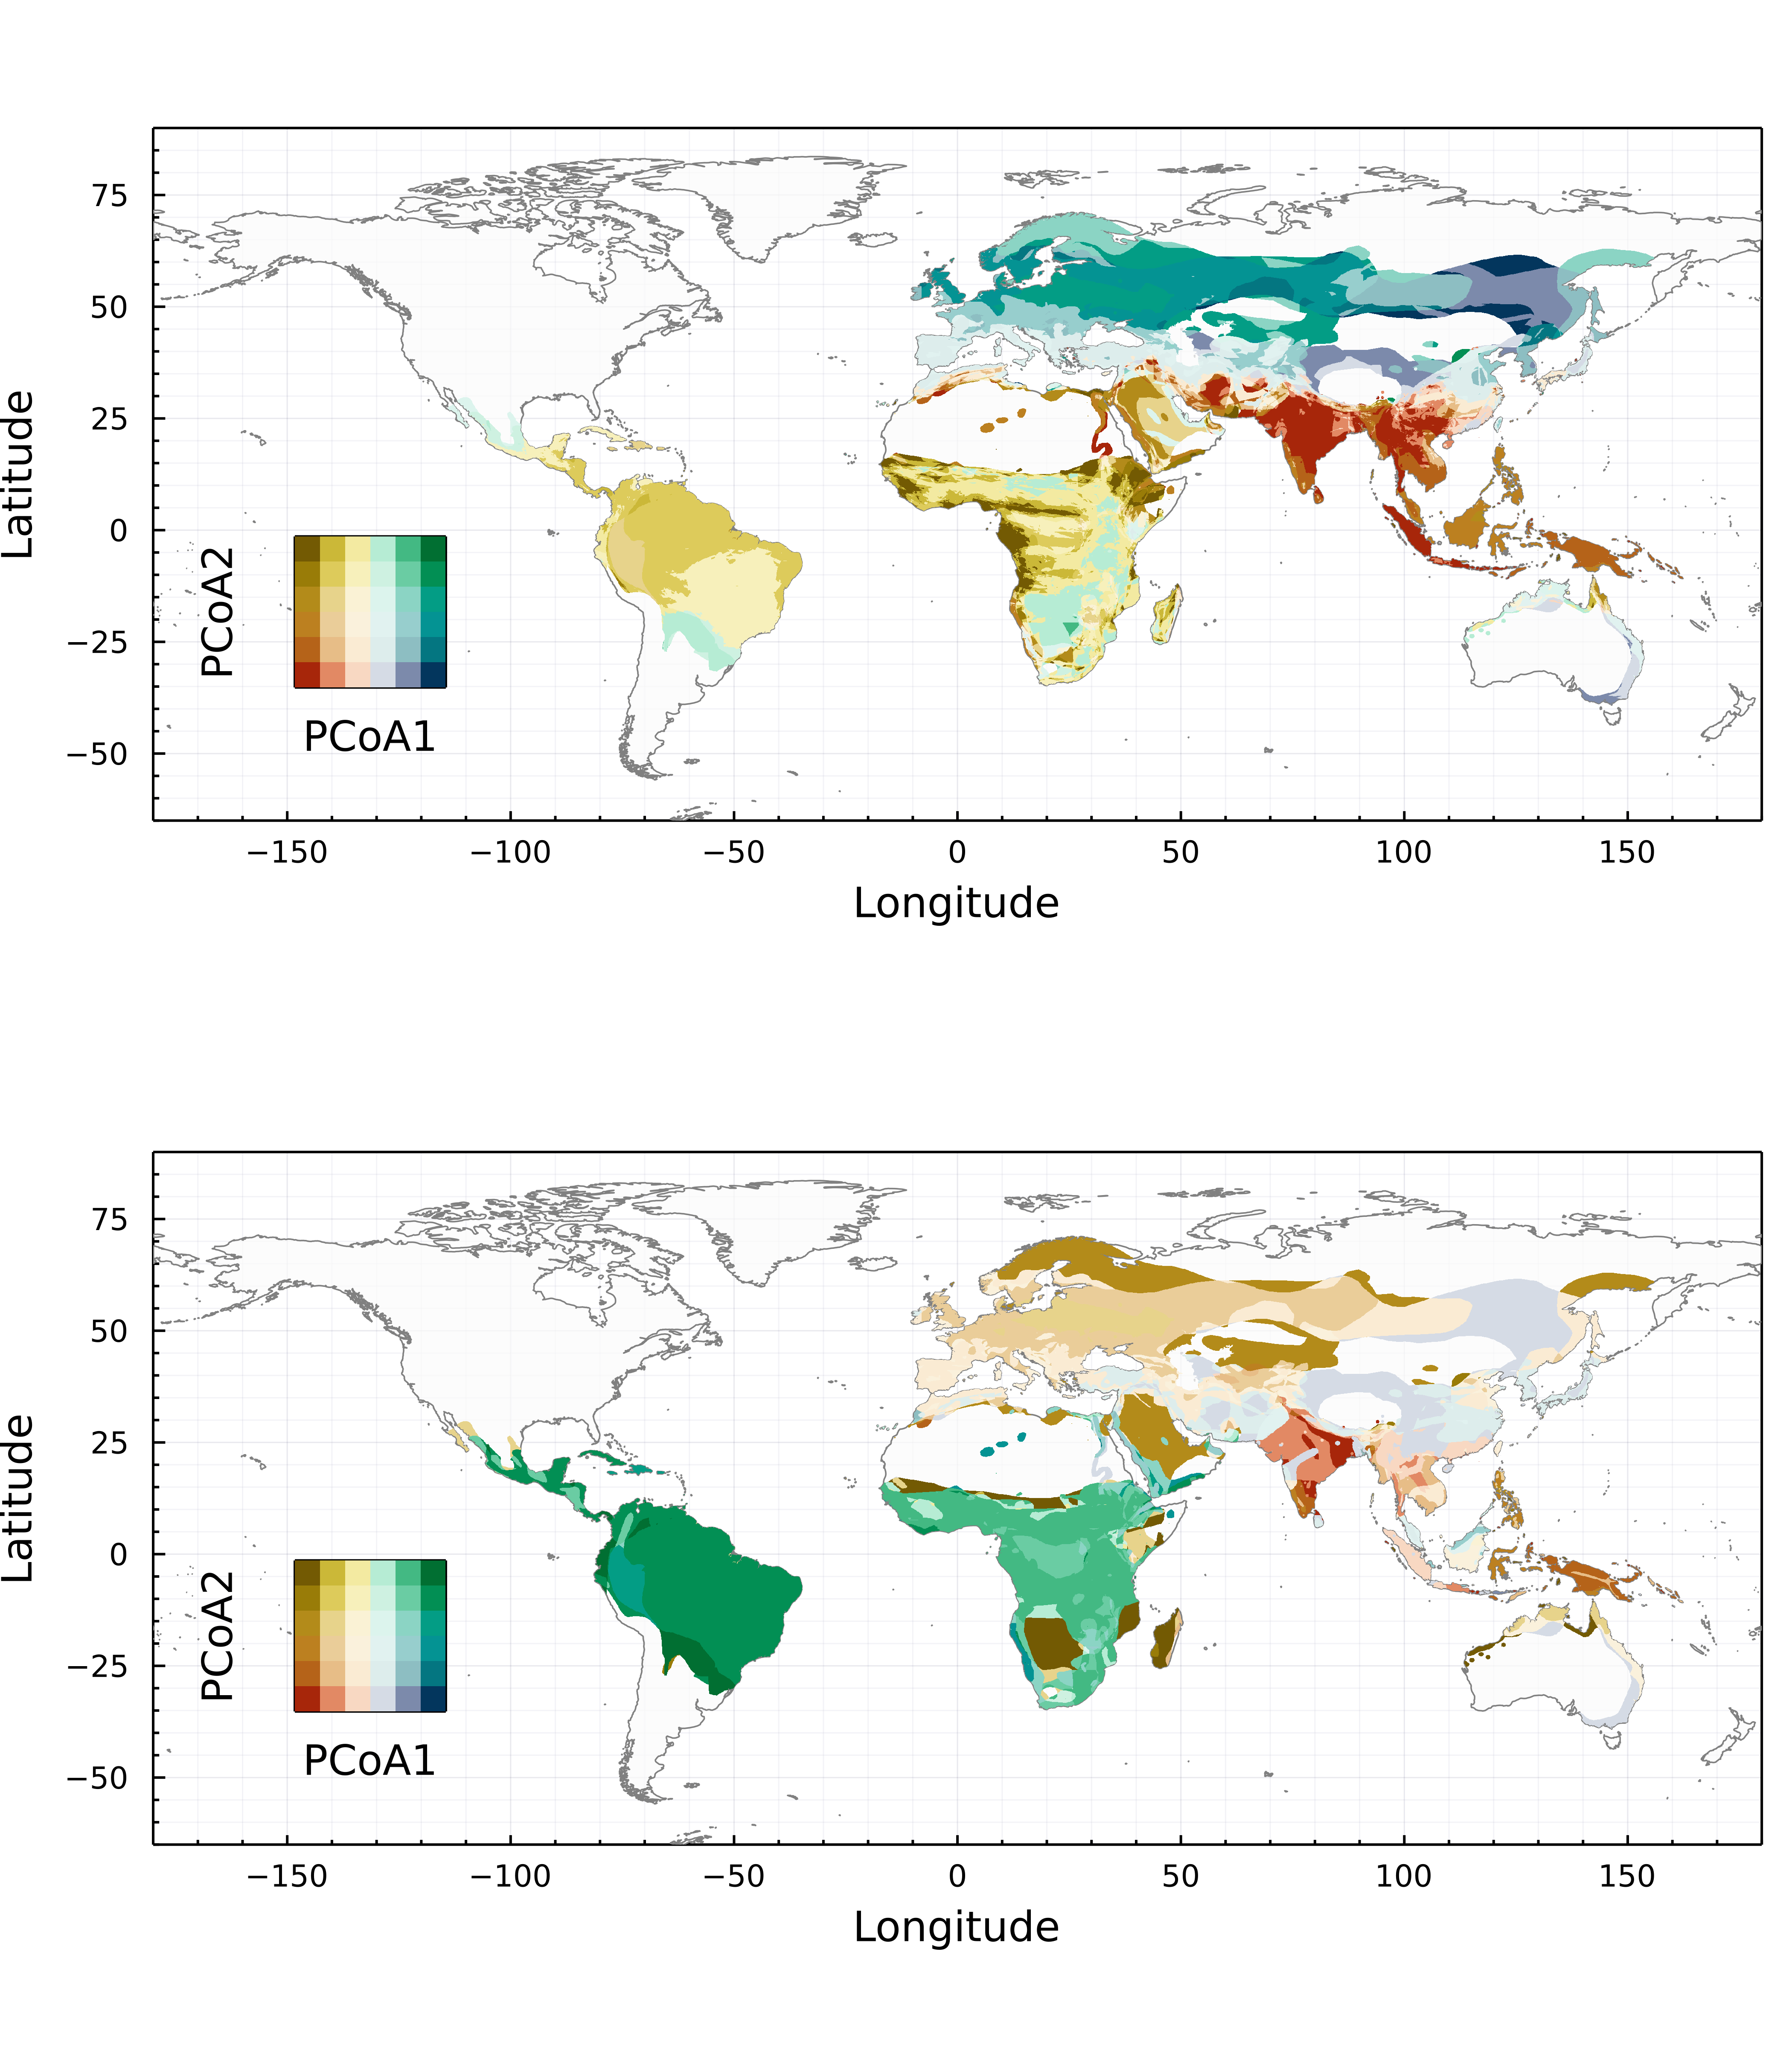
\includegraphics{figures/combined_biogeo.png}
\caption{\textbf{Bat and betacoronavirus biogeographic regions.}
Phylogeography of bats (top) and viruses (bottom) is categorized based
on analysis of bat distributions paired with bat or virus phylogeny. The
different colors show tendencies to separate alongside the first two
components of a PCoA. Note that the PCoA for the bats and viruses are
independent, and so cannot be compared directly -- that being said, the
regions can be compared across maps.}\label{fig:biogeo}
}
\end{figure}

Overall, these results suggest that the boundaries of bat and
betacoronavirus biogeographic regions are largely consistent. This may
be surprising, given that cross-species transmission may play a stronger
role in coronavirus diversification than
cospeciation---\textsuperscript{2}a property that would theoretically
allow for substantial broad divergence in their biogeography. However,
host jumps at the family level or higher are relatively rare and
significant events in coronavirus evolutionary
history;\textsuperscript{2,13} as a result, the mosaic of
betacoronavirus phylogeography is assembled from a set of overlapping
smaller coevolutionary systems, superimposed in space and filtered by
the importance of different subgroups in local host communities. For
example, the most speciose and cosmopolitan family of bats, the vesper
bats (Vespertilionidae), are considered the primary hosts of the
subgenus \emph{Merbecovirus} (MERS-like viruses);\textsuperscript{3,13}
but in the Americas, where merbecoviruses are the only lineage present,
they have only been found in other bat taxa (\emph{e.g.}, Molossidae,
Phyllostomidae).\textsuperscript{14--17} At the coarsest scale, these
heterogeneities are lost, and betacoronavirus biogeography tracks the
deep rifts in bat evolutionary history---but within broad regions, the
component coevolutionary systems may have very different dynamics.

\hypertarget{hotspots-of-bat-and-betacoronavirus-biodiversity-are-distinct}{%
\subsection{Hotspots of bat and betacoronavirus biodiversity are
distinct}\label{hotspots-of-bat-and-betacoronavirus-biodiversity-are-distinct}}

Bats, the second most diverse groups of mammals, are found worldwide;
gradients in their species richness generally track broader patterns of
mammal diversity, with a striking Neotropical hotspot (especially in the
Amazon basin) and a secondary hotspot centered in the southeast Asian
peninsula. These hotspots of bat diversity are generally presumed to be
hotspots of viral adaptive radiation, and therefore areas of concern for
human health.\textsuperscript{2,18} However, the hotspots of known bat
betacoronavirus hosts show a distinct pattern, with primary hotspots
(both in terms of size and higher values) of host richness situated in
southeast Asia, parts of southern Europe, and to a lesser extent parts
of Africa in the -25-0 range of latitudes (fig.~\ref{fig:richness};
top). Although hundreds of species likely host undiscovered
betacoronaviruses, machine learning predictions have suggested that
these undiscovered reservoirs should follow the same diversity
gradient.\textsuperscript{19} In principle, these hotspots of
locally-diverse, virus-rich bat communities should drive more adaptive
diversification in their viruses.

\begin{figure}
\hypertarget{fig:richness}{%
\centering
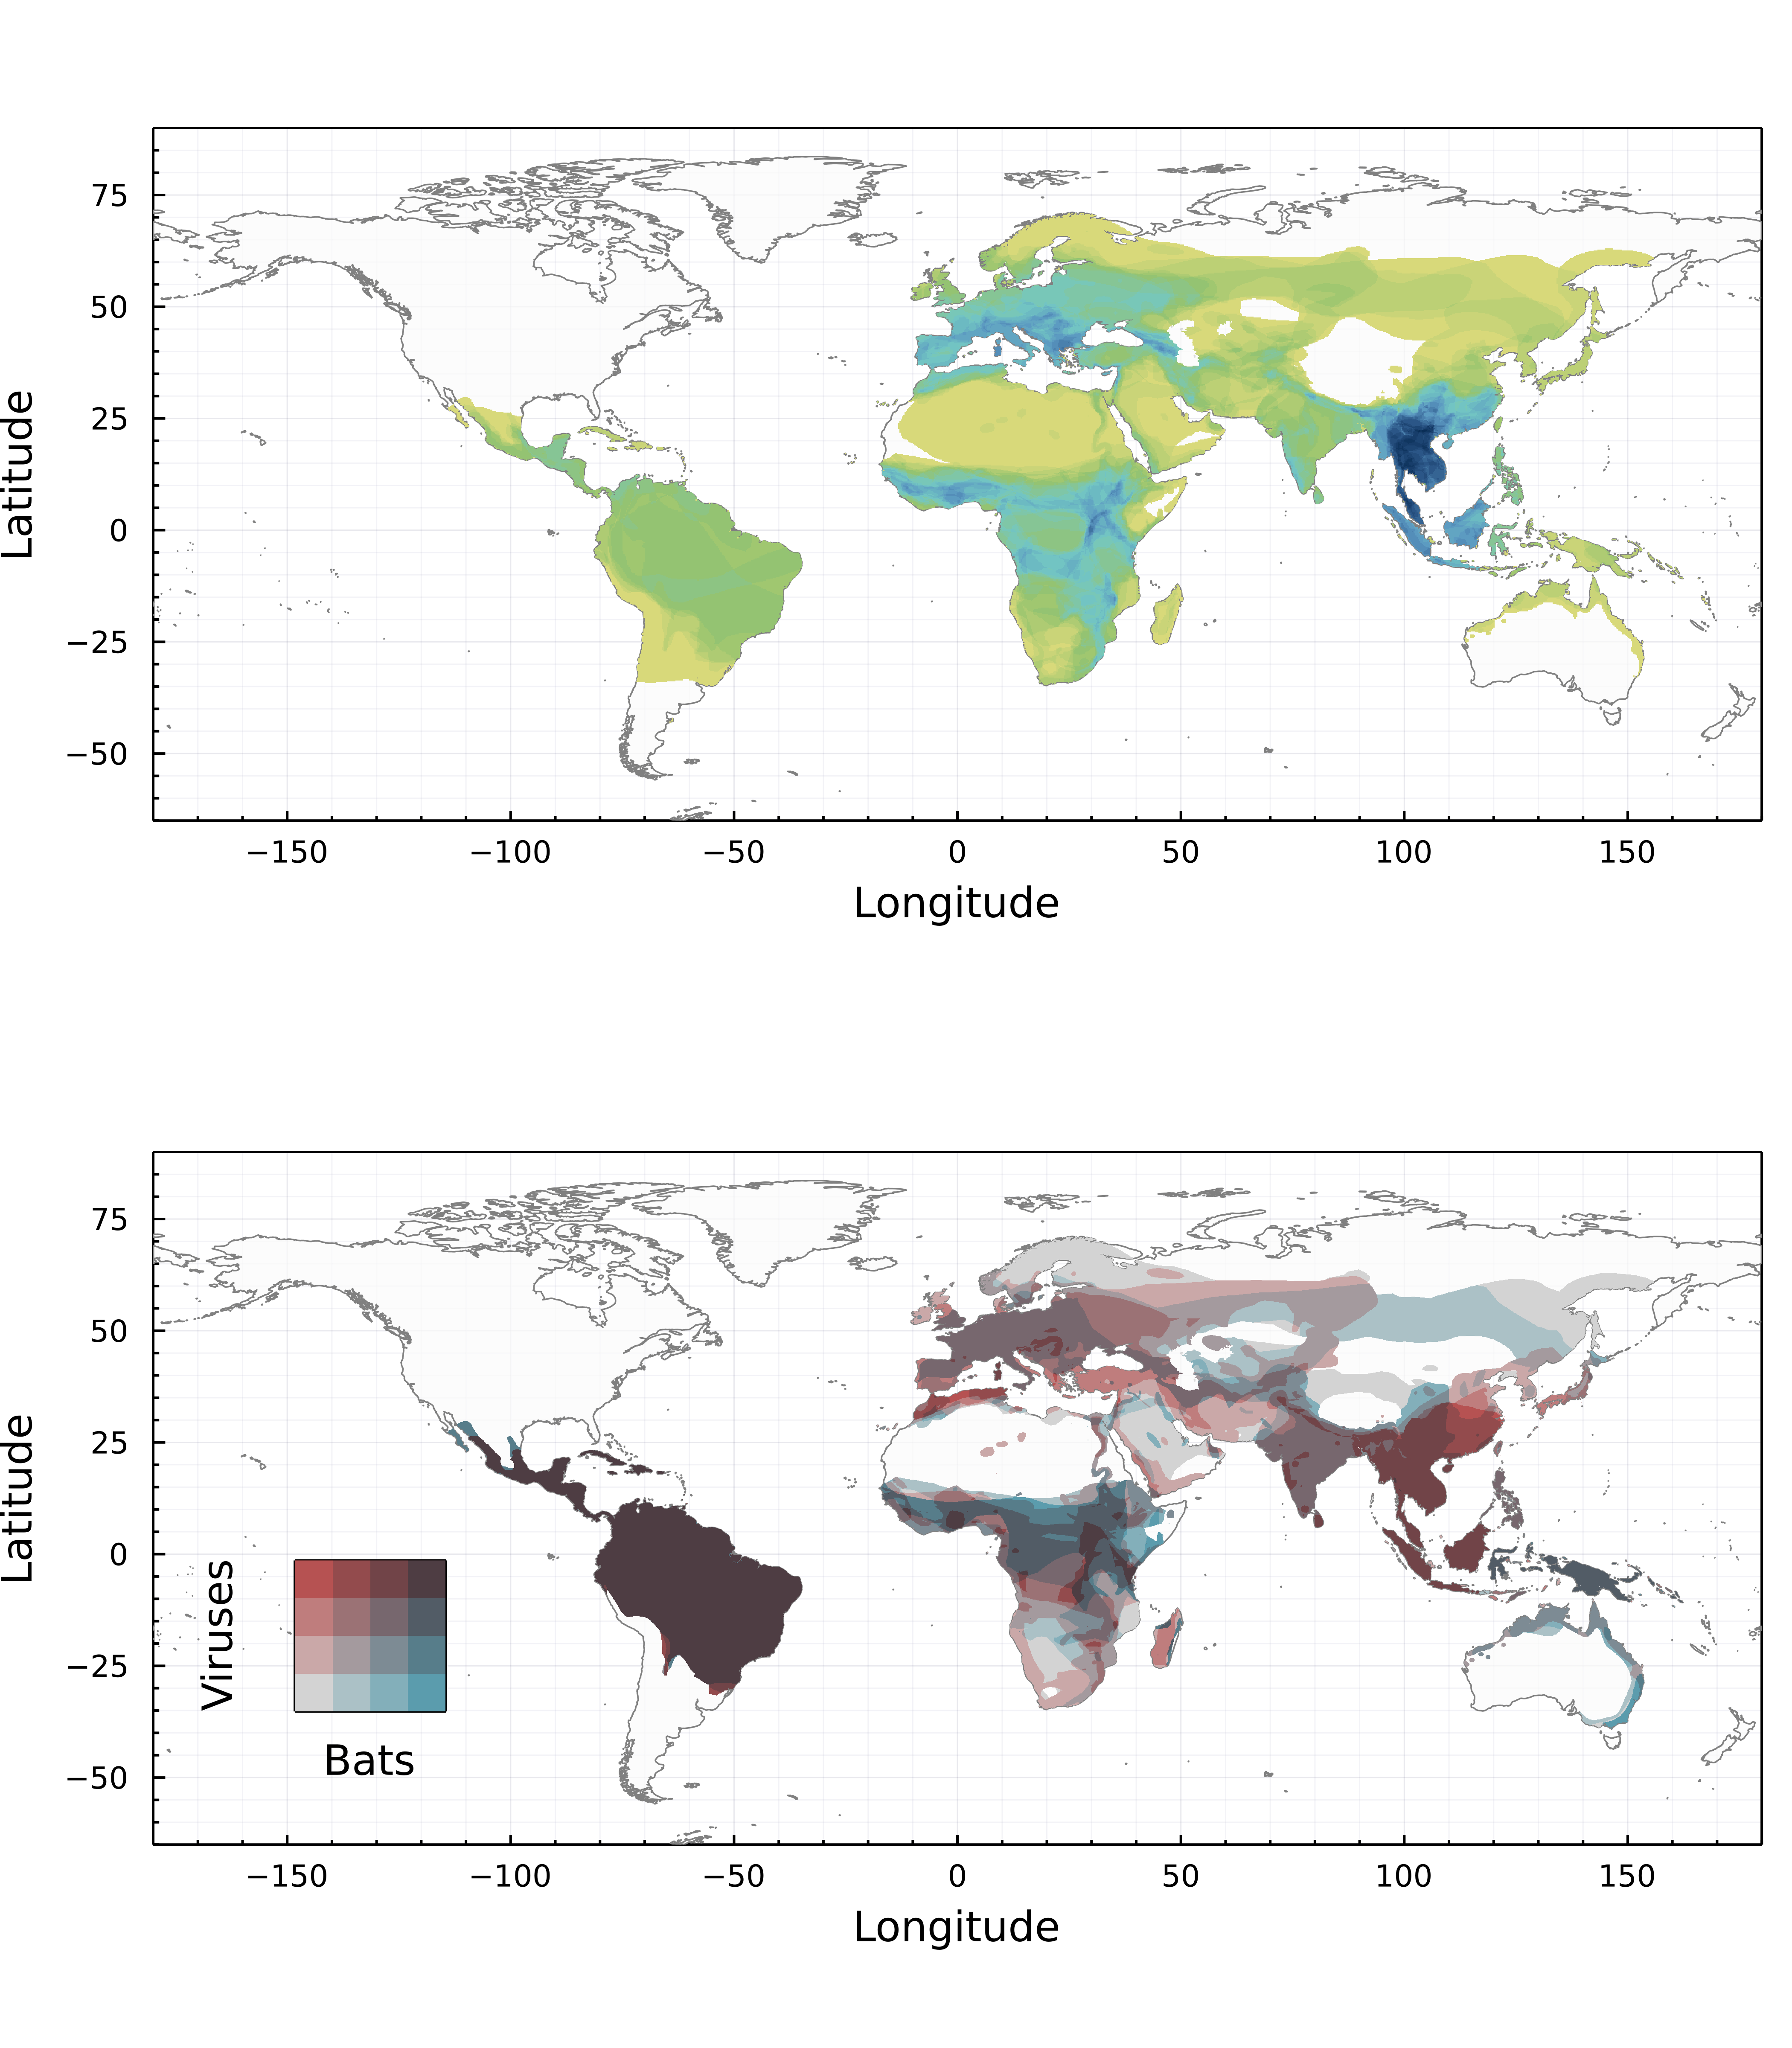
\includegraphics{figures/combined_richness.png}
\caption{\textbf{Bat and betacoronavirus diversity.} Top panel: relative
diversity of known bat hosts of betacoronaviruses. This map shows that
the region with the largest number of possible hosts is South-Eastern
Asia. Bottom panel: congruence between the evolutionary distinctiveness
of the hosts (grey to blue) and the viruses (grey to
red).}\label{fig:richness}
}
\end{figure}

However, we find that the global pattern of betacoronavirus phylogenetic
distinctiveness is quite distinct from both bat host richness and
phylogenetic distinctiveness (fig.~\ref{fig:richness}; bottom). In
contrast to the sparsity of Neotropical betacoronavirus hosts, South and
Central America have the most evolutionary distinct hosts \emph{and}
viruses, followed by secondary hotspots in southeast Asia and the Rift
Valley region have mostly distinct viruses. Some degree of sampling bias
may contribute to these patterns: for example, the Neotropics are one of
the places where the fewest bat betacoronavirus sequences have been
generated (cite2), resulting in a sparser phylogenetic tree, and
artificially inflating distinctiveness; conversely, disproportionate
research effort in eastern China\textsuperscript{20} may have led to a
more complete inventory of the local diversity of coronaviruses, again
inflating these metrics relative to underlying patterns. Even accounting
for these potential biases, though, there is obvious heterogeneity in
betacoronavirus evolutionary distinctiveness that is distinct from
overall bat diversity.

Overall, these patterns recapitulate the evolutionary history of both
the order Chiroptera and the genus \emph{Betacoronavirus}. Horseshoe
bats (Rhinolophidae) include the reservoirs of the SARS-like viruses
(subgenus \emph{Sarbecovirus}), the group of pandemic threats that have
been of the greatest interest to researchers\textsuperscript{13} (and so
have been sampled most intensively).\textsuperscript{20} The hotspots of
host richness and viral diversity in southeast Asia---both of which are
disproportionately high, considering the global landscape of bat species
richness---are almost entirely driven by viral adaptive radiation
through host switching within this clade\textsuperscript{3,19}. In
contrast, the Neotropical hotspot of viral distinctiveness is driven by
isolation by host vicariance. Out of the four main groups of
betacoronaviruses, only merbecoviruses have been found in animals in the
Americas--- an introduction that is generally presumed to be
ancient.\textsuperscript{3,21} While comparatively understudied, New
World merbecoviruses have been found in the ghost-faced bats
(Mormoopidae), Neotropical leaf-nosed bats (Phyllostomidae), and
free-tailed bats (Molossidae).\textsuperscript{14--17} The former two
groups and a clade of the latter are endemic to the Neotropics, while
the explosive adaptive radiations of the phyllostomids are responsible
for the hotspot of bat diversity in the Amazon.\textsuperscript{22}
Together, these clades of New World bats play host to a distinct regime
of betacoronavirus coevolution.

\hypertarget{coevolutionary-regimes-structure-evolutionary-potential-for-zoonotic-emergence}{%
\subsection{Coevolutionary regimes structure evolutionary potential for
zoonotic
emergence}\label{coevolutionary-regimes-structure-evolutionary-potential-for-zoonotic-emergence}}

The existence of well-defined cophylogenetic regions suggests that the
bat-betacoronavirus system is spatially fragmented enough to create
divergent coevolutionary trajectories; in turn, this coevolutionary
mosaic may alter the risk of zoonotic emergence. These ideas are,
respectively, supported by the existence of hotspots of viral uniqueness
and the diverse origins of human betacoronaviruses. Together, this
framework points to a predictable relationship between host community
structure and coevolutionary pressure: phylogeographic structure in bat
hosts (and their diverse immune strategies)\textsuperscript{23} creates
a landscape of selective pressure; the trajectory of viruses'
coevolutionary response is, in turn, constrained by their opportunities
for either specialization or diversification through host jumps and
recombination.

Based on the geographic mosaic theory of coevolution, we developed a
trivariate map of three facets of coevolutionary pressure
(fig.~\ref{fig:trivariate}): (1) \emph{host phylogenetic diversity}: a
high diversity of evolutionary histories should expose viruses to more
variation in host immune traits; (2) \emph{host community uniqueness}:
exposure to greater host trait heterogeneity can drive viral
diversification, and coevolving with more unique host communities should
create more unique branches of viral evolution; and (3) propensity for
\emph{viral sharing}: frequent cross-species transmission may act as a
buffer on selective pressure, while lower rates of exchange may enable
more simultaneous trajectories of viral specialization to coexist within
a given community. We combine global maps of all three to generate a map
of coevolutionary regimes, where close colors represent similar risks,
and paler pixels represent overall higher risk (see Methods). We find
that these regions do not neatly overlap with those defined in
fig.~\ref{fig:biogeo} or fig.~\ref{fig:richness}, reinforcing the notion
that local-scale coevolutionary mosaics can form within cophylogenetic
regions.

\begin{figure}
\hypertarget{fig:trivariate}{%
\centering
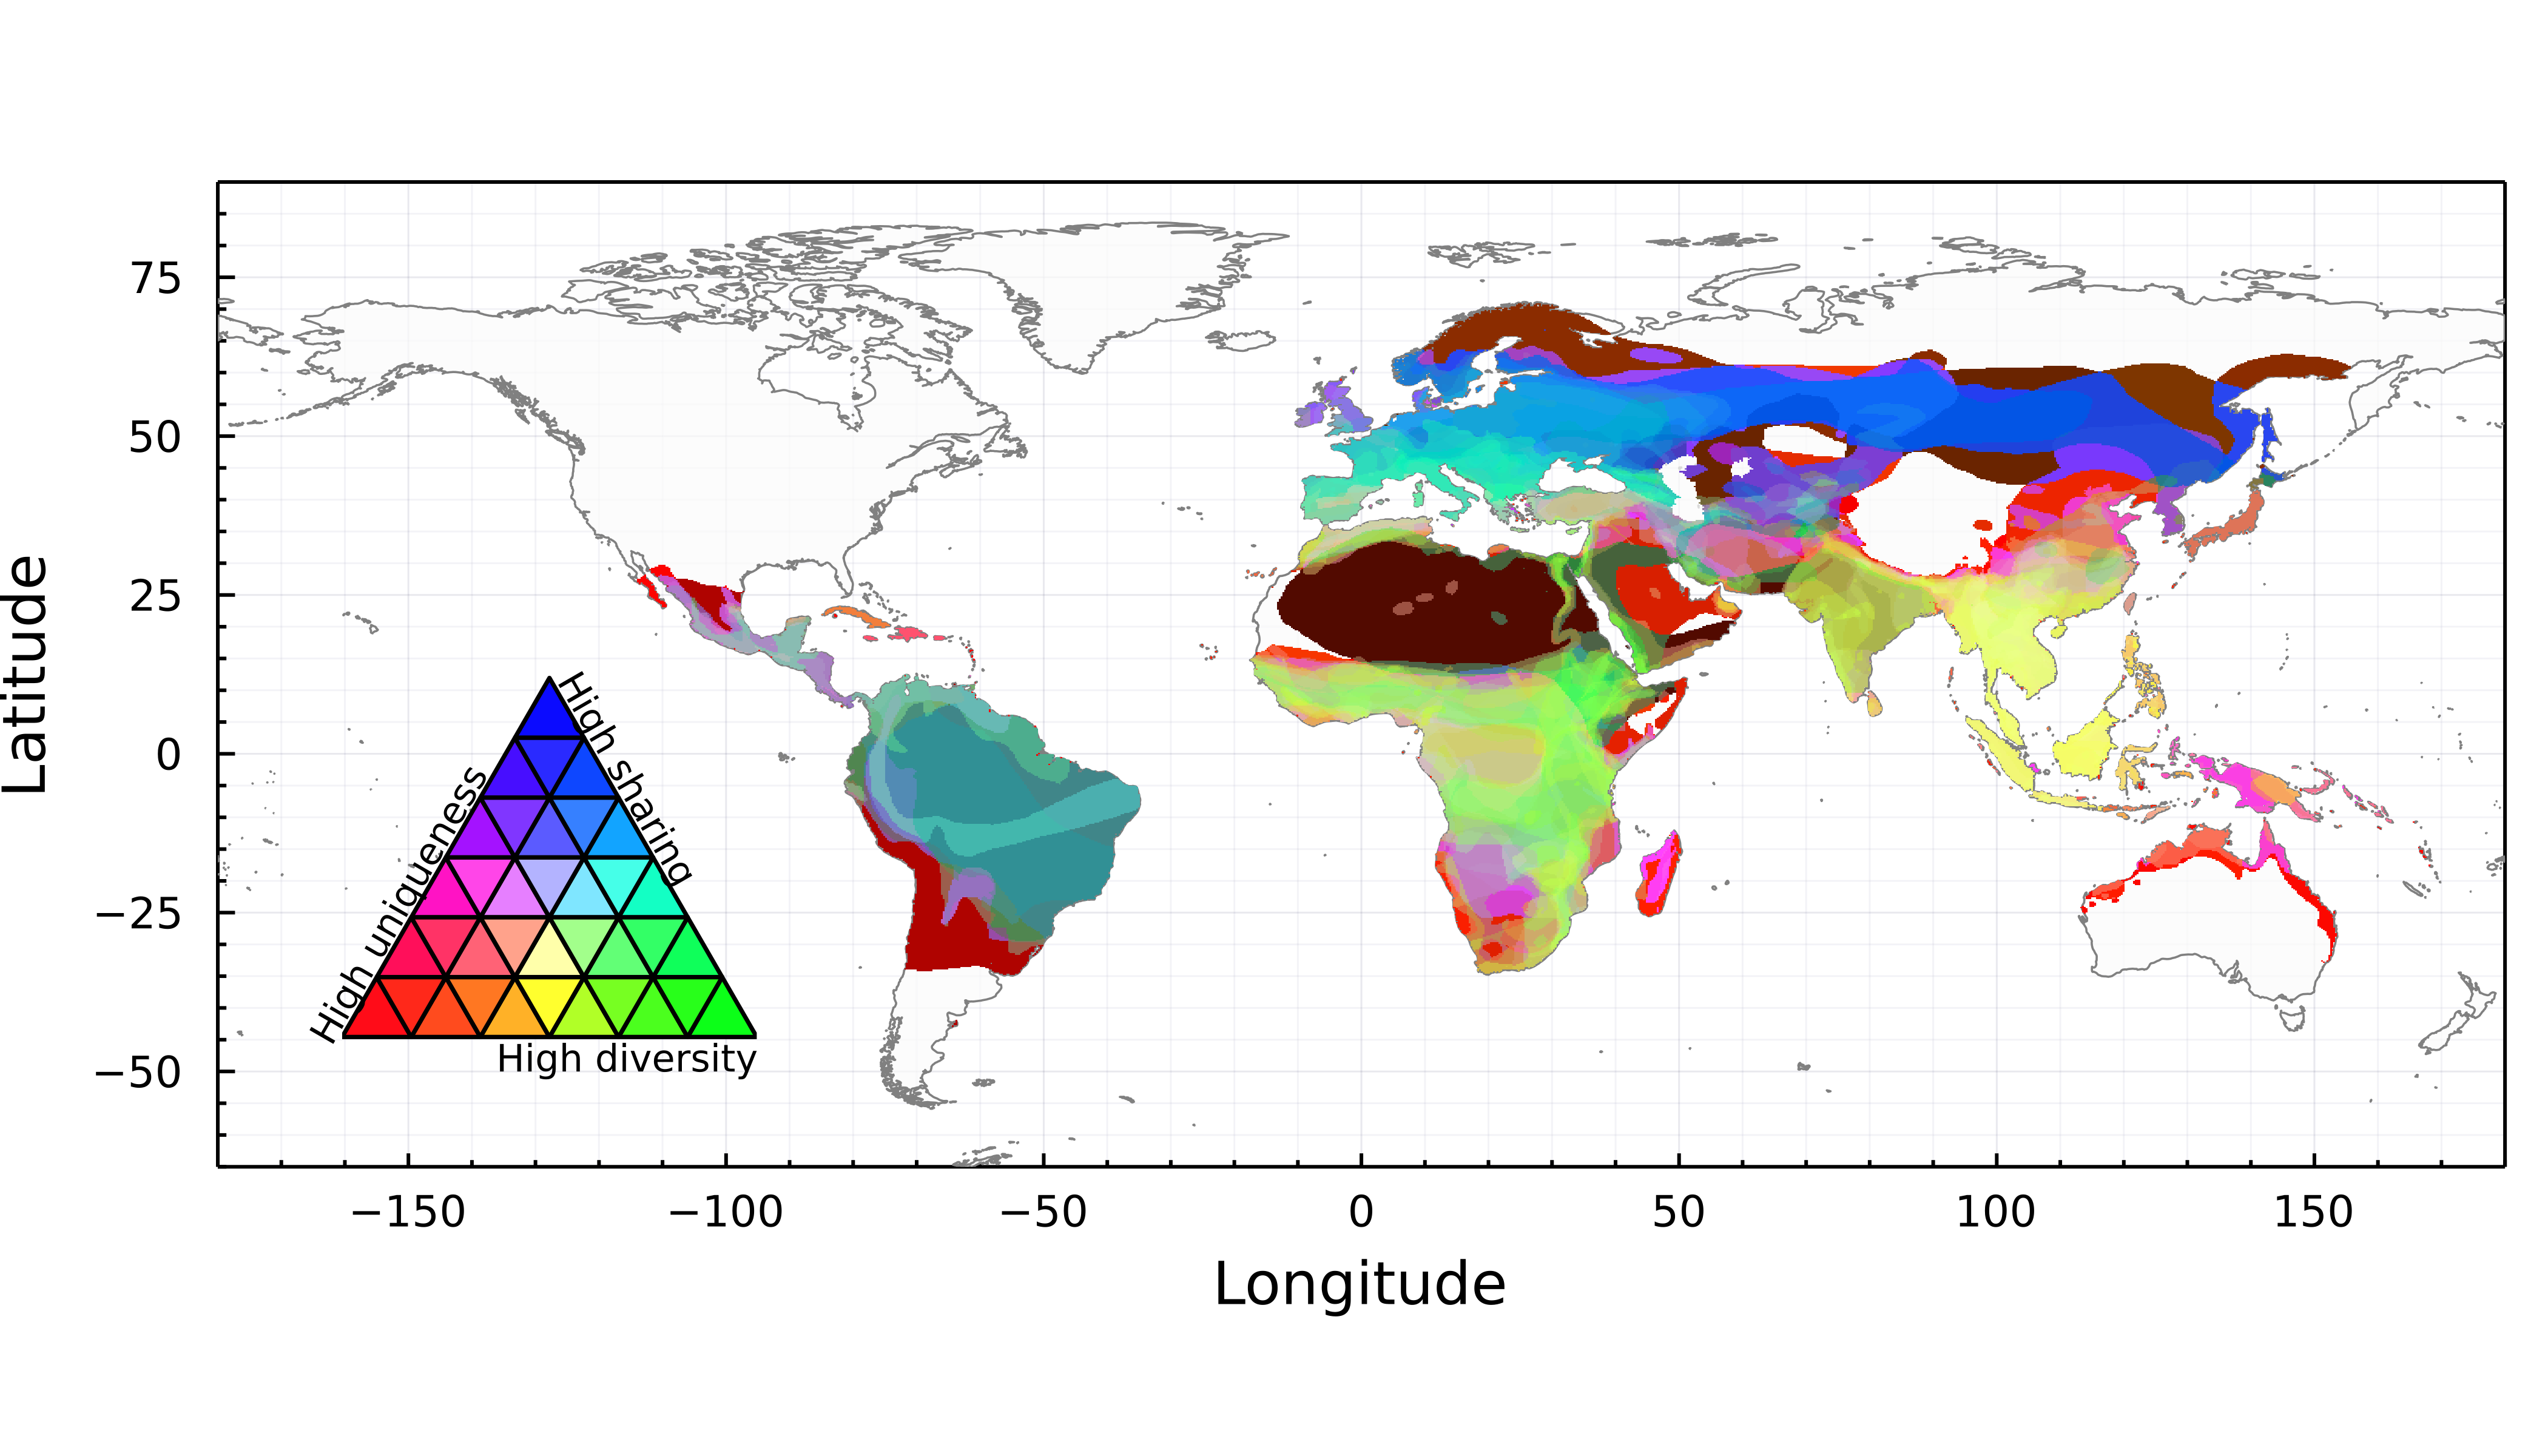
\includegraphics{figures/risk_trivariate.png}
\caption{\textbf{Trivariate additive mapping of the components of risk.}
Viral sharing runs from yellow (low) to blue (high); host phylogenetic
diversity runs from pink (low) to high (green); and host compositional
uniqueness runs from cyan (low) to red (high). The GMTC suggests that
the highest evolutionary potential for emergence exists in unique and
diverse host communities with low viral sharing, \emph{i.e.} pixels
around yellow. All components are scaled in brightness so that a pixel
with no sharing, no phylogenetic diversity, and no compositional
uniqueness would be black, and a pixel with maximal values for each
would be white.}\label{fig:trivariate}
}
\end{figure}

The greatest evolutionary potential for zoonotic emergence exists where
pathogen pools have a high genetic diversity and high propensity for
cross-species transmission. In our framework, emergence risk is
therefore maximized under higher phylogenetic diversity (viruses are
exposes to different host clades), higher host uniqueness (viruses are
experiencing novel, heterogeneous host traits combinations), and low to
medium viral sharing (host-virus pairs can coevolve independently, but
divergent viruses may still have opportunities for recombination). In
fig.~\ref{fig:trivariate}, this corresponds to yellow areas (dynamics
dominated by low viral sharing, with equal contributions of selection
mosaics and trait remixing; southeast Asia, and the Indian
sub-continent), green-yellow areas (dynamics with low viral sharing but
dominated by the selection mosaic effect of host diversity; sub-Saharan
Africa), and red-yellow areas (dynamics with low viral sharing but
dominated by trait remixing in host communities; the Middle East).
Translating this axis of variation back into a univariate risk map
(fig.~\ref{fig:risk}) highlights that this evolutionary landscape has a
striking correspondence to regions where zoonotic betacoronaviruses have
previously emerged.

Compared to approaches that map emergence risk based only on the number
of known bat hosts of betacoronaviruses, our framework suggests regions
where high viral sharing dominates coevolutionary dynamics---such as
Latin America, or Eurasia above a northing of 30---would pose less of a
relative risk of zoonotic emergence. Nevertheless, areas of high host
uniqueness coupled with high viral sharing (red-to-pink in
fig.~\ref{fig:trivariate}) could create hotspots facilitated by viral
codivergence. Our framework identifies Madagascar, where most bat
species are endemic following evolutionary divergence from sister
species in both African and Asian continents,\textsuperscript{24} as one
such hotspot; interestingly, a recent study\textsuperscript{25} reported
a novel and highly divergent lineage of nobecoviruses from
Madagascar-endemic pteropid bat species (\emph{Pteropus rufus} and
\emph{Rousettus madagascariensis}), again supporting the predictive
power of the coevolutionary framework.

\begin{figure}
\hypertarget{fig:risk}{%
\centering
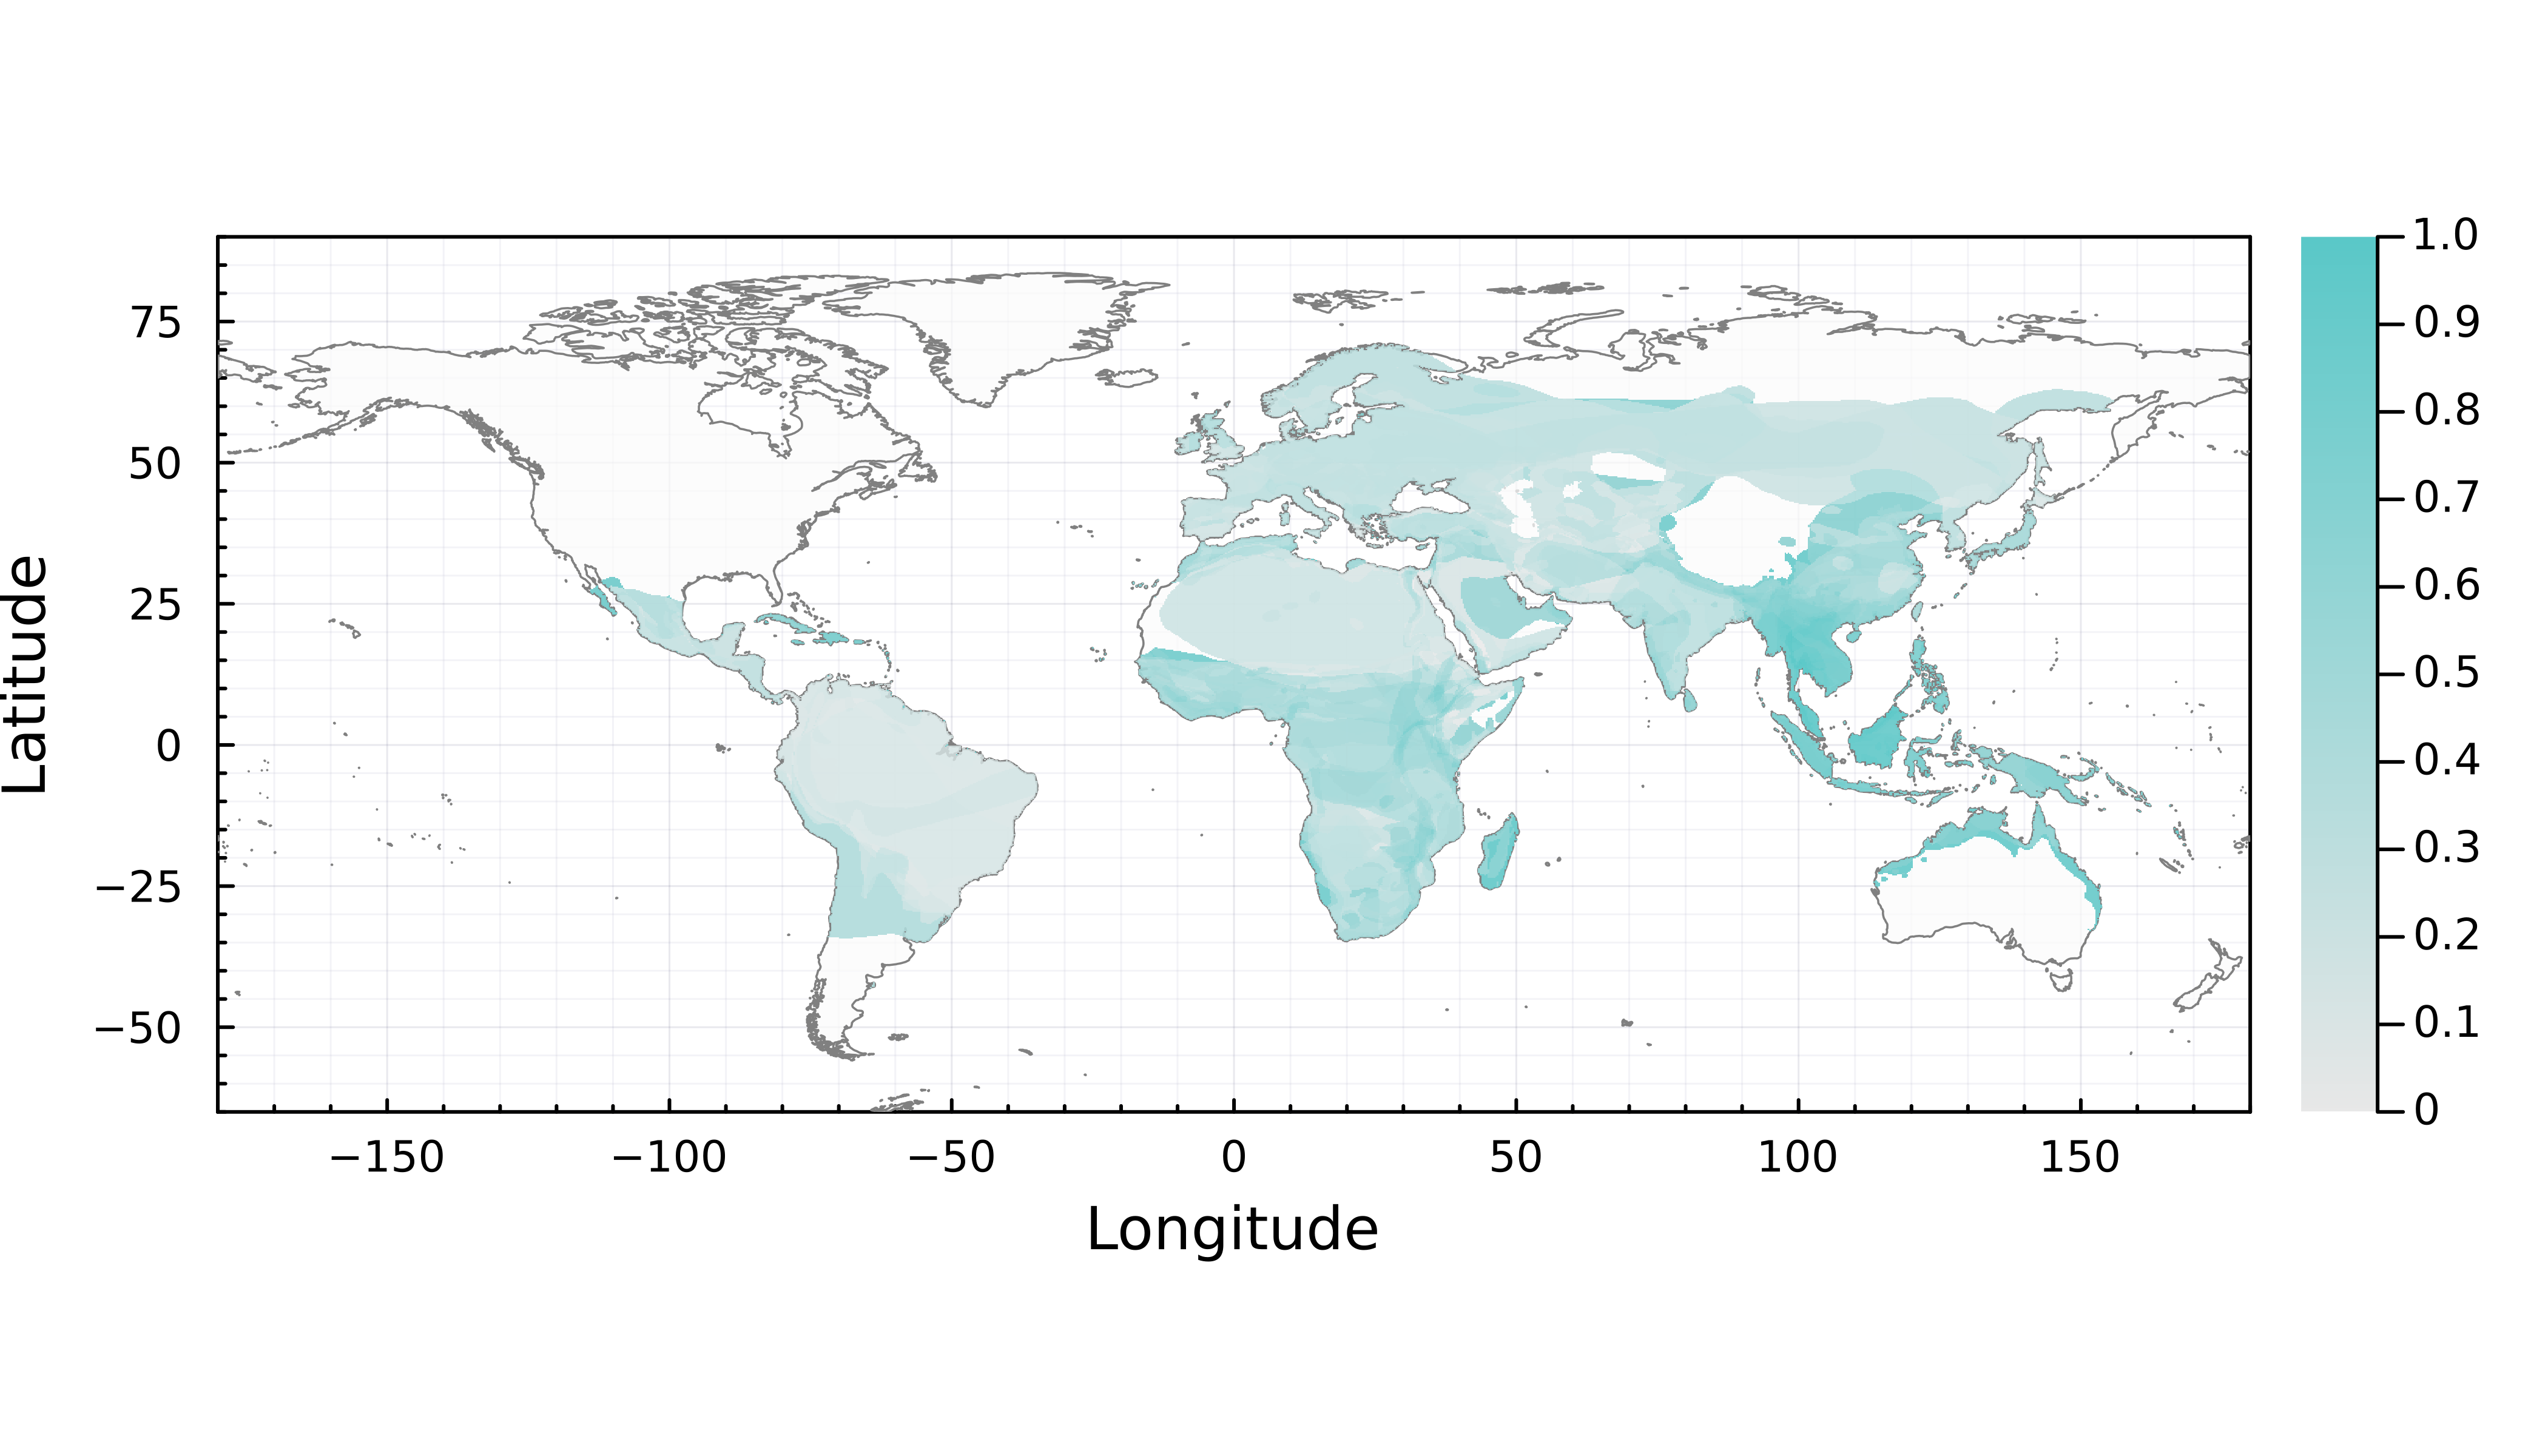
\includegraphics{figures/risk_map.png}
\caption{\textbf{Evolutionary potential for zoonotic emergence of
bat-origin betacoronaviruses.} Risk is a composite measure of the color
value and angular distance to the yellow hue in
fig.~\ref{fig:trivariate} (see Methods).}\label{fig:risk}
}
\end{figure}

\hypertarget{human-landscapes-filter-the-geography-of-emergence-risk}{%
\subsection{Human landscapes filter the geography of emergence
risk}\label{human-landscapes-filter-the-geography-of-emergence-risk}}

The relationship between the underlying pathogen pool and emergence risk
is mediated by both human-wildlife interfaces (the probability of
spillover) and opportunities for onward transmission (the probability
that spillovers become epidemics)\textsuperscript{1}. As a proxy for
both, we finally overlaid the risk component from the composite map (see
above) with the proportion of built land, as a proxy for a mix of
habitat disturbance, potential for bat synanthropy or contact with
bridge hosts like livestock,\textsuperscript{26,27} and human population
density and connectivity\textsuperscript{1,28,29}
(fig.~\ref{fig:compound}). Accounting for these factors, most of South
America and Europe are at comparatively lower risk, as--although densely
populated--settlements tend to be in areas with lower potential risk.
Conversely, regions like Malaysia and the northern coast of Australia
have a high evolutionary risk component, but should represent a
relatively lower effective risk due to low human density. However,
southeast Asia, the Indian subcontinent, and scattered hotspots in
sub-Saharan Africa are at high risk due to the overlap between human
populations and natural opportunities for cross-species transmission of
betacoronaviruses.

\begin{figure}
\hypertarget{fig:compound}{%
\centering
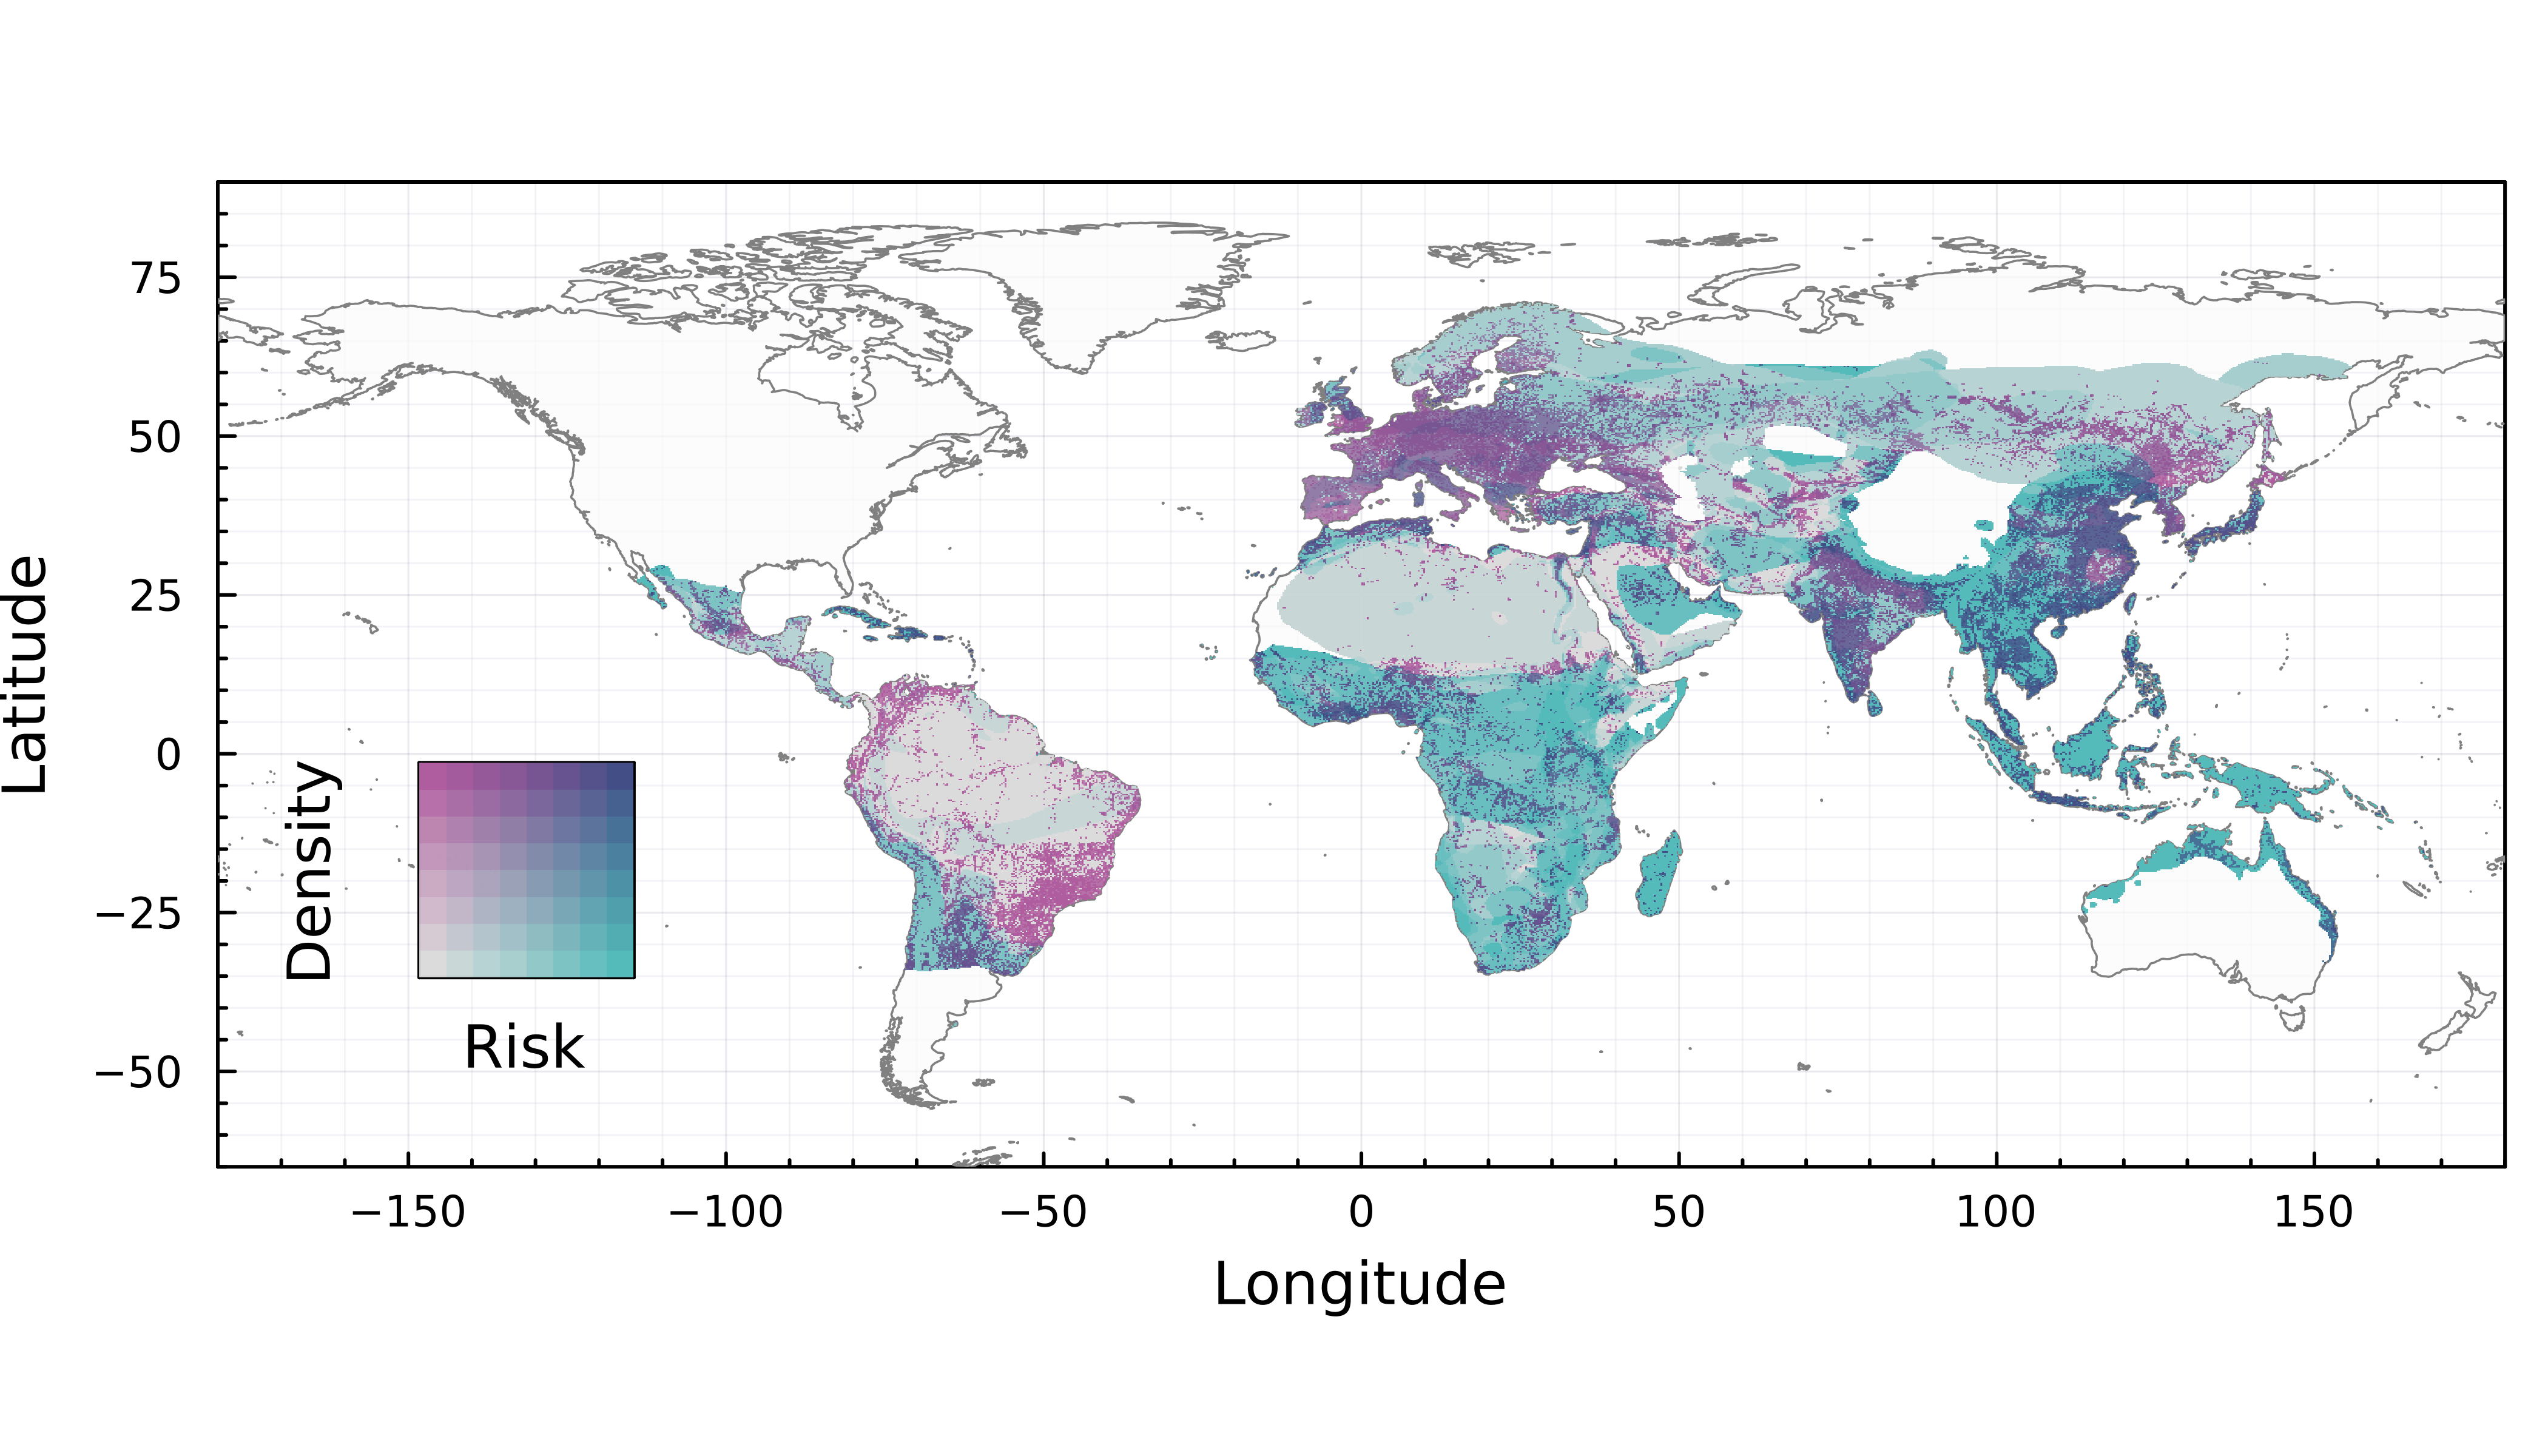
\includegraphics{figures/risk_compounded.png}
\caption{\textbf{Overlap between evolutionary potential and ecological
opportunity for zoonotic emergence.} Overlap of the percent of each
pixel occupied by urbanized structures, representing the degree of
settlement, on the spillover risk map (where the risk comes only from
wildlife, and ignores multi-hosts chains of transmissions including
non-bats hosts). Darker pixels correspond to more risk, in that the
GMTC-derived risk of fig.~\ref{fig:risk} is high \emph{and} the pixel is
densely occupied by human populations.}\label{fig:compound}
}
\end{figure}

Reassuringly, these predictions correspond to the geographic origins of
the three bat-origin coronaviruses that have recently emerged in human
populations. While available information puts the spillover of
SARS-CoV-2 in a live animal market in Wuhan, China, the ultimate origin
of the virus is almost certainly in a divergent lineage of
sarbecoviruses from the Indochinese peninsula that was poorly
characterized prior to the pandemic.\textsuperscript{30--32} Similarly,
the SARS-CoV outbreak began in Guangdong province in 2002, reaching
humans through small carnivore bridge hosts, but was eventually traced
back to a set of likely progenitor viruses found in cave-dwelling
horseshoe bats in Yunnan province;\textsuperscript{33} nearby, antibody
evidence has indicated human exposure to SARS-like
viruses.\textsuperscript{34} MERS-CoV was originally detected in Saudi
Arabia, accompanied by a nearly identical virus sequenced from an
Egyptian tomb bat (\emph{Taphozous perforatus}),\textsuperscript{35} but
is widespread in camels in East Africa and the Middle East, and may have
reached its bridge host decades earlier than originally
supposed;\textsuperscript{36} as a result, the geography of the original
bat-to-camel transmission is still widely regarded as uncertain. All of
these are broadly consistent with the risk factors we identify. Notably,
India and west Africa are additional hotspots that have yet to
experience the emergence of a bat coronavirus into human populations,
but may still be at risk---particularly given known gaps in bat
surveillance,\textsuperscript{20} and a dense population in both regions
with global connectivity. In any of these regions, surveillance on viral
reservoirs can be paired with targeted monitoring of high-risk human
populations (i.e., those with regular wildlife
contact)\textsuperscript{37} for maximum impact.

\hypertarget{conclusion}{%
\section{Conclusion}\label{conclusion}}

Bats emerged around 64 million years ago, and are one of the most
diverse mammalian orders, with more than 1,400 estimated
species.\textsuperscript{38,39} They exhibit a broad variety of habitat
use, behaviour, and feeding strategies, putting them at key positions in
the delivery and provisioning of several ecosystem services, tied to
important ecosystem-derived benefits to humans.\textsuperscript{40} Over
two-thirds of bats are know to be either obligate or facultative
insectivores, therefore actively contributing for agricultural pest
control,\textsuperscript{41,42} and vectors of pathogens that put a risk
on human health;\textsuperscript{43,44} some other species are essential
links in many seed-dispersal networks.\textsuperscript{45} However, many
of these species face a high risk of extinction, particularly given
persecution and killings that sometimes follows from messaging about
their role in disease emergence. Areas where bats, viruses, and humans
co-occur are not always hotspots of risk for human heath; as such,
developing more precise ways to map zoonotic hazards can help bats and
humans coexist safely, and support the conservation of these important
and unique animals.

Here, we propose a simple framework with broad explanatory power that
helps contextualize discoveries like highly divergent nobecoviruses in
Madagascar and the once-neglected adaptive radiation of sarbecoviruses
in the Indochinese peninsula. In doing so, it advances ecological theory
beyond the current state of the art for global maps of emergence risk.
For example, previous studies that have used host richness as a proxy
have predicted a high diversity of unsampled bat
viruses,\textsuperscript{18} bat coronaviruses,\textsuperscript{2} and
even specifically betacoronaviruses\textsuperscript{19} in both the
Amazon and southeast Asia. While we find that both regions are
characterized by unique and diverse communities of both hosts and
viruses, our framework is able to identify key differences between the
two systems. We find that the merbecovirus complex in Latin America has
been a unique branch of evolution separate from the rest of the global
pool, but with limited potential for viral diversification--- a finding
that is supported by previous work indicating a higher rate of
codivergence in Latin America.\textsuperscript{2} In contrast, in
southeast Asia, host richness and viral distinctiveness are high but
sharing is low; this suggests a different type of evolutionary dynamics
that could generate high local diversity of viruses through host
switching and viral recombination (see \emph{e.g.},\textsuperscript{13}
as well as the discovery of recombinant viruses with genetic material
from both the SARS-CoV and SARS-CoV-2 branches of the Sarbecovirus
lineage).\textsuperscript{46}

Both of these regions are priority areas for sampling, especially given
predictions that they contain many bat hosts of undiscovered
betacoronaviruses.\textsuperscript{19,20} However, both the evolutionary
and ecological aspects of emergence risk are higher in southeast
Asia---a fact that will only become more relevant, as bats track
shifting climates and exchange viruses with other species, creating a
hotspot of elevated cross-species transmission unique to the
region.\textsuperscript{28,47} Bats---and the spillover of their
viruses---are also sensitive to anthropogenic factors others than
climate change, including deforestation and other kinds of habitat loss,
increased stress, and greater contact with potential bridge hosts like
domesticated species\textsuperscript{26,48,49} (add cite for
10.1038/nature13139). This represents a challenge for both conservation
strategies and pandemic prevention,\textsuperscript{50} but identifying
areas at risk, and protecting the health of bats and ecosystems within
those zones, can be a win-win intervention for both (add cites for DOIs:
10.1038/s41893-020-00640-z; 10.1016/S2542-5196(21)00031-0).

\textbf{Acknowledgements}: We acknowledge that this study was conducted
on land within the traditional unceded territory of the Saint Lawrence
Iroquoian, Anishinabewaki, Mohawk, Huron-Wendat, and Omàmiwininiwak
nations. This work was supported by funding to the Viral Emergence
Research Initiative (VERENA) consortium including NSF BII 2021909 and a
grant from Institut de Valorisation des Données (IVADO). This research
was enabled in part by support provided by Calcul Québec
(www.calculquebec.ca) and Compute Canada (www.computecanada.ca). NF is
funded by the NSERC BIOS² CREATE program. TP and NF are funded by the
Courtois Foundation. RLM was supported by Bryce Carmine and Anne Carmine
(née Percival), through the Massey University Foundation. DJB was
supported by the National Institute of General Medical Sciences of the
National Institutes of Health (P20GM134973).

\newpage

\hypertarget{methods}{%
\section{Methods}\label{methods}}

\hypertarget{known-betacoronavirus-hosts}{%
\subsection{\texorpdfstring{Known \emph{Betacoronavirus}
hosts}{Known Betacoronavirus hosts}}\label{known-betacoronavirus-hosts}}

We downloaded the data on bats hosts of \emph{Betacoronavirus} from
\texttt{https://www.viralemergence.org/betacov} on
Apr.~2022,\textsuperscript{19} and filtered it to ``known'' hosts
(established before the emergence of SARS-CoV-2) and ``novel'' hosts
(confirmed through sampling and competence assays since the initial data
collection). The original database was assembled by a combination of
data mining and literature surveys, including automated alerts on the
``bats'' and ``coronavirus'' keywords to identify novel empirical
evidence of bats-betacoronaviruses associations; this yielded a total of
126 known hosts, 47 of which were novel hosts.

\hypertarget{bat-occurrences}{%
\subsection{Bat occurrences}\label{bat-occurrences}}

We downloaded the rangemap of every current bat species that was
classified as an empirically documented host of \emph{Betacoronavirus}
from the previous step, according to recent IUCN
data.\textsuperscript{51} The range maps were subsequently rasterized
using the \texttt{rasterize} function from
\texttt{GDAL}\textsuperscript{52} at a resolution of approximately
100kmx100km. For every pixel in the resulting raster where at least one
bat host of \emph{Betacoronavirus} was present, we extract the species
pool (list of all known bat hosts), which was used to calculate the
following risk assessment components: bat phylogenetic diversity, bat
compositional uniqueness, and predicted viral sharing risk.

\hypertarget{bat-phylogenetic-diversity}{%
\subsection{Bat phylogenetic
diversity}\label{bat-phylogenetic-diversity}}

For every pixel, we measured Faith's Phylogenetic
Diversity\textsuperscript{53} based on a recent synthetic tree with
robust time calibration, covering about 6000 mammalian
species.\textsuperscript{54} Faith's PD measures the sum of unique
branches from an arbitrary root to a set of tips, and comparatively
larger values indicate a more phylogenetic diverse species pool. We
measured phylogenetic diversity starting from the root of the entire
tree (and not from Chiroptera); this bears no consequences on the
resulting values, since all branches leading up to Chiroptera are only
counted one per species pool, and (as we explain when describing the
assembly of the composite risk map), all individual risk components are
ranged in {[}0,1{]}. This measure incorporates a richness component,
which we chose not to correct for; the interpretation of the
phylogenetic diversity is therefore a weighted species richness, that
accounts for phylogenetic over/under-dispersal in some places.

\hypertarget{bat-compositional-uniqueness}{%
\subsection{Bat compositional
uniqueness}\label{bat-compositional-uniqueness}}

For every species pool, we measured its Local Contribution to
Beta-Diversity;\textsuperscript{55} LCBD works from a species-data
matrix (traditionally noted as \(\mathbf{Y}\)), where species are rows
and sites are columns, and a value of 1 indicates occurrence. We
extracted the Y matrix assuming that every pixel represents a unique
location, and following best practices\textsuperscript{56} transformed
it using Hellinger's distance to account for unequal bat richness at
different pixels. The correction of raw community data is particularly
important for two reasons: first, it prevents the artifact of richer
sites having higher importance; second, it removes the effect of overall
species richness, which is already incorporated in the phylogenetic
diversity component. High values of LCBD indicate that the pixel has a
community that is on average more dissimilar in species composition than
what is expected knowing the entire matrix, i.e.~a more unique
community. Recent results by\textsuperscript{57} shows that LCBD
measures are robust with regards to spatial scale, and are therefore
applicable at the global scale.

\hypertarget{viral-sharing-between-hosts}{%
\subsection{Viral sharing between
hosts}\label{viral-sharing-between-hosts}}

For all bat hosts of \emph{Betacoronavirus}, we extracted their
predicted viral sharing network, generated from a previously published
generalized additive mixed model of virus sharing by a tensor function
of phylogenetic distance and geographic range overlap across
mammals.\textsuperscript{58} This network stores pairwise values of
viral community similarity. To project viral sharing values into a
single value for every pixel, we averaged the pairwise scores. High
values of the average sharing propensity means that this specific extant
bat assemblage is likely to be proficient at exchanging viruses.

\hypertarget{composite-risk-map}{%
\subsection{Composite risk map}\label{composite-risk-map}}

To visualize the aggregated risk at the global scale, we combine the
three individual risk components (phylogenetic diversity, compositional
uniqueness, and viral sharing) using an additive color
model.\textsuperscript{59} In this approach, every risk component gets
assigned a component in the RGB color model (phylogenetic diversity is
green, compositional uniqueness is red, and viral sharing is blue). In
order to achieve a valid RGB measure, all components are re-scaled to
the {[}0,1{]} interval, so that a pixel with no sharing, no phylogenetic
diversity, and no compositional uniqueness is black, and a pixel with
maximal values for each is white. This additive model conveys both the
intensity of the overall risk, but also the nature of the risk as colors
diverge towards combinations of values for three risk components. Out of
the possible combinations, the most risky in terms or rapid
diversification and spillover potential is high phylogenetic diversity
and low viral sharing,\textsuperscript{60} in that this allows multiple
independent host-virus coevolutionary dynamics to take place in the same
location. In the colorimetric space, this correspond to yellow --
because the HSV space is more amenable to calculations for feature
extraction,\textsuperscript{61} we measured the risk level by
calculating the angular distance of the hue of each pixel to a reference
value of 60 (yellow), and weighted this risk level by the value
component. Specifically, given a pixel with colorimetric coordinates
\((h,s,v)\), its ranged weighted risk value is

\[
v\times\left[1-\frac{\left|\text{atan}\left(\text{cos}(\text{rad}(h)), \text{sin}(\text{rad}(h))\right) - X\right|}{2\pi}\right]\,,
\]

where X is
\(\text{atan}\left(\text{cos}(\text{rad}(60)), \text{sin}(\text{rad}(60))\right)\),
a constant approximately equal to \(0.5235\).

\hypertarget{viral-phylogeography-and-evolutionary-diversification}{%
\subsection{Viral phylogeography and evolutionary
diversification}\label{viral-phylogeography-and-evolutionary-diversification}}

To next represent phylogeography of betacoronaviruses in bats, we
aggregated and analyzed betacoronavirus sequence data. We used the
following query to pull all \emph{Betacoronavirus} sequence data from
the GenBank Nucleotide database except SARS-CoV-2;
(``Betacoronavirus''{[}Organism{]} OR betacoronavirus{[}All Fields{]})
NOT (``Severe acute respiratory syndrome coronavirus 2''{[}Organism{]}
OR sars-cov-2{[}All Fields{]}). We added a single representative
sequence for SARS-CoV-2 and manually curated to remove sequences without
the RNA-dependent RNA polymerase (RdRp) sequence or that contained words
indicating recombinant or laboratory strains including ``patent'',
``mutant'', ``GFP'', and ``recombinant''. We filtered over-represented
taxa including betacoronavirus 1, hCoV-OC43, Middle East respiratory
syndrome coronavirus, Murine hepatitis virus, and hCoV-HKU1. Curated
betacoronavirus RdRp sequences were then aligned using
MAFFT\textsuperscript{62} v1.4.0 (Algorithm FFT-NS-2, Scoring matrix
200PAM / k=2, gap open penalty 1.53m offset value 0.123) and a maximum
likelihood tree reconstructed in IQ-TREE\textsuperscript{63} v1.6.12
with ModelFinder\textsuperscript{64} ultrafast bootstrap
approximation\textsuperscript{65} with a general time reversible model
with empirical base frequencies and the 5-discrete-rate-category
FreeRaye model of nucleotide substitution (GTR+F+R5).

We first tested the hypothesis that hotspots of viral diversification
would track hotspots of bat diversification. To do so, we plotted the
number of known bat hosts (specifically only those included in the
phylogeny, so there was a 1:1 correspondence between data sources)
against the ``mean evolutionary distinctiveness'' of the associated
viruses. To calculate this, we derived the fair proportions evolutionary
distinctiveness\textsuperscript{66} for each of the viruses in the tree,
then averaged these at the bat species level, projected these values
onto their geographic distributions, and averaged across every bat found
in a given pixel. As such, this can be thought of as a map of the mean
evolutionary distinctiveness of the known viral community believed to be
associated with a particular subset of bats present.

\hypertarget{co-distribution-of-hosts-and-viral-hotspots}{%
\subsection{Co-distribution of hosts and viral
hotspots}\label{co-distribution-of-hosts-and-viral-hotspots}}

Subsequently, we tested the hypothesis that the biogeography of bat
betacoronaviruses should track the biogeography of their hosts. To test
this idea, we loosely adapted a method from,\textsuperscript{67,68} who
proposed a phylogenetic method for the delineation of animal
biogeographic regions. In their original method, a distance matrix -
where each row or column represents a geographic raster's grid cell, and
the dissimilarity values are the ``beta diversity similarity'' of their
community assemble - undergoes non-metric multidimensional scaling
(NMDS); the first two axes of the NMDS are projected geographically
using a four-color bivariate map. Here, we build on this idea with an
entirely novel methodology. First, we measure the phylogenetic distance
between the different viruses in the betacoronaviruses tree by using the
cophenetic function in \texttt{ape};\textsuperscript{69} subsequently,
we take a principal components analysis of that distance matrix (readily
interchangeable for NMDS in this case) to project the viral tree into an
n-dimensional space. We then take the first two principal components
and, as with the evolutionary distinctiveness analysis, aggregated these
to a mean host value and projected them using a four-color bivariate
map.

\newpage

\hypertarget{references}{%
\section*{References}\label{references}}
\addcontentsline{toc}{section}{References}

\hypertarget{refs}{}
\begin{CSLReferences}{0}{0}
\leavevmode\hypertarget{ref-Plowright2017PatZoo}{}%
\CSLLeftMargin{1. }
\CSLRightInline{Plowright, R. K. \emph{et al.} Pathways to zoonotic
spillover. \emph{Nature Reviews Microbiology} \textbf{15}, 502--510
(2017).}

\leavevmode\hypertarget{ref-Anthony2017GloPat}{}%
\CSLLeftMargin{2. }
\CSLRightInline{Anthony, S. J. \emph{et al.} Global patterns in
coronavirus diversity. \emph{Virus Evolution} \textbf{3}, (2017).}

\leavevmode\hypertarget{ref-Ruiz-Aravena2022EcoEvo}{}%
\CSLLeftMargin{3. }
\CSLRightInline{Ruiz-Aravena, M. \emph{et al.} Ecology, evolution and
spillover of coronaviruses from bats. \emph{Nature Reviews Microbiology}
\textbf{20}, 299--314 (2022).}

\leavevmode\hypertarget{ref-Agosta2010HowSpe}{}%
\CSLLeftMargin{4. }
\CSLRightInline{Agosta, S. J., Janz, N. \& Brooks, D. R. How specialists
can be generalists: Resolving the {`parasite paradox'} and implications
for emerging infectious disease. \emph{Zoologia (Curitiba)} \textbf{27},
151--162 (2010).}

\leavevmode\hypertarget{ref-Power2004PatSpi}{}%
\CSLLeftMargin{5. }
\CSLRightInline{Power, A. G. \& Mitchell, C. E. Pathogen Spillover in
Disease Epidemics. \emph{The American Naturalist} \textbf{164}, S79--S89
(2004).}

\leavevmode\hypertarget{ref-Geoghegan2017ComAna}{}%
\CSLLeftMargin{6. }
\CSLRightInline{Geoghegan, J. L., Duchêne, S. \& Holmes, E. C.
Comparative analysis estimates the relative frequencies of co-divergence
and cross-species transmission within viral families. \emph{PLOS
Pathogens} \textbf{13}, e1006215 (2017).}

\leavevmode\hypertarget{ref-Thompson2005GeoMos}{}%
\CSLLeftMargin{7. }
\CSLRightInline{Thompson, J. N. \emph{The Geographic Mosaic of
Coevolution}. (University Of Chicago Press, 2005).}

\leavevmode\hypertarget{ref-Thompson1994CoePro}{}%
\CSLLeftMargin{8. }
\CSLRightInline{Thompson, J. N. \emph{The Coevolutionary Process}.
(University of Chicago Press, 1994).}

\leavevmode\hypertarget{ref-Janzen1980WheIt}{}%
\CSLLeftMargin{9. }
\CSLRightInline{Janzen, D. H. When is it Coevolution? \emph{Evolution}
\textbf{34}, 611--612 (1980).}

\leavevmode\hypertarget{ref-Price2002MacThe}{}%
\CSLLeftMargin{10. }
\CSLRightInline{Price, P. W. \emph{Macroevolutionary Theory on
Macroecological Patterns}. (Cambridge University Press, 2002).
doi:\href{https://doi.org/10.1017/CBO9780511615030}{10.1017/CBO9780511615030}.}

\leavevmode\hypertarget{ref-Gomulkiewicz2007DosDon}{}%
\CSLLeftMargin{11. }
\CSLRightInline{Gomulkiewicz, R. \emph{et al.} Dos and don'ts of testing
the geographic mosaic theory of coevolution. \emph{Heredity}
\textbf{98}, 249--258 (2007).}

\leavevmode\hypertarget{ref-Thrall2007CoeSym}{}%
\CSLLeftMargin{12. }
\CSLRightInline{Thrall, P. H., Hochberg, M. E., Burdon, J. J. \& Bever,
J. D. Coevolution of symbiotic mutualists and parasites in a community
context. \emph{Trends in Ecology \& Evolution} \textbf{22}, 120--126
(2007).}

\leavevmode\hypertarget{ref-Latinne2020OriCro}{}%
\CSLLeftMargin{13. }
\CSLRightInline{Latinne, A. \emph{et al.} Origin and cross-species
transmission of bat coronaviruses in China. \emph{bioRxiv: The Preprint
Server for Biology} 2020.05.31.116061 (2020)
doi:\href{https://doi.org/10.1101/2020.05.31.116061}{10.1101/2020.05.31.116061}.}

\leavevmode\hypertarget{ref-Anthony2013CorBat}{}%
\CSLLeftMargin{14. }
\CSLRightInline{Anthony, S. J. \emph{et al.} Coronaviruses in bats from
Mexico. \emph{The Journal of General Virology} \textbf{94}, 1028--1038
(2013).}

\leavevmode\hypertarget{ref-Goes2013NovBat}{}%
\CSLLeftMargin{15. }
\CSLRightInline{Góes, L. G. B. \emph{et al.} Novel Bat Coronaviruses,
Brazil and Mexico. \emph{Emerging Infectious Diseases} \textbf{19},
1711--1713 (2013).}

\leavevmode\hypertarget{ref-Goes2016GenDiv}{}%
\CSLLeftMargin{16. }
\CSLRightInline{Góes, L. G. B. \emph{et al.} Genetic diversity of bats
coronaviruses in the Atlantic Forest hotspot biome, Brazil.
\emph{Infection, Genetics and Evolution: Journal of Molecular
Epidemiology and Evolutionary Genetics in Infectious Diseases}
\textbf{44}, 510--513 (2016).}

\leavevmode\hypertarget{ref-Brandao2008CorDet}{}%
\CSLLeftMargin{17. }
\CSLRightInline{Brandão, P. E. \emph{et al.} A coronavirus detected in
the vampire bat Desmodus rotundus. \emph{Brazilian Journal of Infectious
Diseases} \textbf{12}, 466--468 (2008).}

\leavevmode\hypertarget{ref-Olival2017HosVir}{}%
\CSLLeftMargin{18. }
\CSLRightInline{Olival, K. J. \emph{et al.} Host and viral traits
predict zoonotic spillover from mammals. \emph{Nature} \textbf{546},
646--650 (2017).}

\leavevmode\hypertarget{ref-Becker2022OptPre}{}%
\CSLLeftMargin{19. }
\CSLRightInline{Becker, D. J. \emph{et al.} Optimising predictive models
to prioritise viral discovery in zoonotic reservoirs. \emph{The Lancet
Microbe} (2022)
doi:\href{https://doi.org/10.1016/S2666-5247(21)00245-7}{10.1016/S2666-5247(21)00245-7}.}

\leavevmode\hypertarget{ref-Cohen2022SamStr}{}%
\CSLLeftMargin{20. }
\CSLRightInline{Cohen, L. E., Fagre, A. C., Chen, B., Carlson, C. J. \&
Becker, D. J. Sampling strategies and pre-pandemic surveillance gaps for
bat coronaviruses. 2022.06.15.496296 (2022)
doi:\href{https://doi.org/10.1101/2022.06.15.496296}{10.1101/2022.06.15.496296}.}

\leavevmode\hypertarget{ref-Olival2020PosRev}{}%
\CSLLeftMargin{21. }
\CSLRightInline{Olival, K. J. \emph{et al.} Possibility for reverse
zoonotic transmission of SARS-CoV-2 to free-ranging wildlife: A case
study of bats. \emph{PLoS pathogens} \textbf{16}, e1008758 (2020).}

\leavevmode\hypertarget{ref-Ammerman2012FirMol}{}%
\CSLLeftMargin{22. }
\CSLRightInline{Ammerman, L. K., Lee, D. N. \& Tipps, T. M. First
molecular phylogenetic insights into the evolution of free-tailed bats
in the subfamily Molossinae (Molossidae, Chiroptera). \emph{Journal of
Mammalogy} \textbf{93}, 12--28 (2012).}

\leavevmode\hypertarget{ref-Banerjee2020NovIns}{}%
\CSLLeftMargin{23. }
\CSLRightInline{Banerjee, A. \emph{et al.} Novel Insights Into Immune
Systems of Bats. \emph{Frontiers in Immunology} \textbf{11}, 26 (2020).}

\leavevmode\hypertarget{ref-Shi2014DeeDiv}{}%
\CSLLeftMargin{24. }
\CSLRightInline{Shi, J. J. \emph{et al.} A Deep Divergence Time between
Sister Species of Eidolon (Pteropodidae) with Evidence for Widespread
Panmixia. \emph{Acta Chiropterologica} \textbf{16}, 279--292 (2014).}

\leavevmode\hypertarget{ref-Kettenburg2022FulGen}{}%
\CSLLeftMargin{25. }
\CSLRightInline{Kettenburg, G. \emph{et al.} Full Genome Nobecovirus
Sequences From Malagasy Fruit Bats Define a Unique Evolutionary History
for This Coronavirus Clade. \emph{Frontiers in Public Health}
\textbf{10}, (2022).}

\leavevmode\hypertarget{ref-Rulli2021LanCha}{}%
\CSLLeftMargin{26. }
\CSLRightInline{Rulli, M. C., D'Odorico, P., Galli, N. \& Hayman, D. T.
Land-use change and the livestock revolution increase the risk of
zoonotic coronavirus transmission from rhinolophid bats. \emph{Nature
Food} \textbf{2}, 409--416 (2021).}

\leavevmode\hypertarget{ref-Cui2019OriEvo}{}%
\CSLLeftMargin{27. }
\CSLRightInline{Cui, J., Li, F. \& Shi, Z.-L. Origin and evolution of
pathogenic coronaviruses. \emph{Nature Reviews Microbiology}
\textbf{17}, 181--192 (2019).}

\leavevmode\hypertarget{ref-Muylaert2022PreFut}{}%
\CSLLeftMargin{28. }
\CSLRightInline{Muylaert, R. L. \emph{et al.} Present and future
distribution of bat hosts of sarbecoviruses: Implications for
conservation and public health. \emph{Proceedings of the Royal Society
B: Biological Sciences} \textbf{289}, 20220397 (2022).}

\leavevmode\hypertarget{ref-Hassell2017UrbDis}{}%
\CSLLeftMargin{29. }
\CSLRightInline{Hassell, J. M., Begon, M., Ward, M. J. \& Fèvre, E. M.
Urbanization and disease emergence: Dynamics at the
wildlife--livestock--human interface. \emph{Trends in ecology \&
evolution} \textbf{32}, 55--67 (2017).}

\leavevmode\hypertarget{ref-Worobey2022HuaMar}{}%
\CSLLeftMargin{30. }
\CSLRightInline{Worobey, M. \emph{et al.} The Huanan market was the
epicenter of SARS-CoV-2 emergence. \emph{Zenodo} (2022)
doi:\href{https://doi.org/10.5281/zenodo.6299600}{10.5281/zenodo.6299600}.}

\leavevmode\hypertarget{ref-Temmam2022BatCor}{}%
\CSLLeftMargin{31. }
\CSLRightInline{Temmam, S. \emph{et al.} Bat coronaviruses related to
SARS-CoV-2 and infectious for human cells. \emph{Nature} \textbf{604},
330--336 (2022).}

\leavevmode\hypertarget{ref-Boni2020EvoOri}{}%
\CSLLeftMargin{32. }
\CSLRightInline{Boni, M. F. \emph{et al.} Evolutionary origins of the
SARS-CoV-2 sarbecovirus lineage responsible for the COVID-19 pandemic.
\emph{Nature microbiology} \textbf{5}, 1408--1417 (2020).}

\leavevmode\hypertarget{ref-Hu2017DisRic}{}%
\CSLLeftMargin{33. }
\CSLRightInline{Hu, B. \emph{et al.} Discovery of a rich gene pool of
bat SARS-related coronaviruses provides new insights into the origin of
SARS coronavirus. \emph{PLoS pathogens} \textbf{13}, e1006698 (2017).}

\leavevmode\hypertarget{ref-Wang2018SerEvi}{}%
\CSLLeftMargin{34. }
\CSLRightInline{Wang, N. \emph{et al.} Serological Evidence of Bat
SARS-Related Coronavirus Infection in Humans, China. \emph{Virologica
Sinica} \textbf{33}, 104--107 (2018).}

\leavevmode\hypertarget{ref-Memish2013MidEas}{}%
\CSLLeftMargin{35. }
\CSLRightInline{Memish, Z. A. \emph{et al.} Middle East respiratory
syndrome coronavirus in bats, Saudi Arabia. \emph{Emerging infectious
diseases} \textbf{19}, 1819 (2013).}

\leavevmode\hypertarget{ref-Muller2014MerCor}{}%
\CSLLeftMargin{36. }
\CSLRightInline{Müller, M. A. \emph{et al.} MERS coronavirus
neutralizing antibodies in camels, Eastern Africa, 1983--1997.
\emph{Emerging infectious diseases} \textbf{20}, 2093 (2014).}

\leavevmode\hypertarget{ref-Xu2004EpiClu}{}%
\CSLLeftMargin{37. }
\CSLRightInline{Xu, R.-H. \emph{et al.} Epidemiologic Clues to SARS
Origin in China. \emph{Emerging Infectious Diseases} \textbf{10},
1030--1037 (2004).}

\leavevmode\hypertarget{ref-Peixoto2018SynEco}{}%
\CSLLeftMargin{38. }
\CSLRightInline{Peixoto, F. P., Braga, P. H. P. \& Mendes, P. A
synthesis of ecological and evolutionary determinants of bat diversity
across spatial scales. \emph{BMC ecology} \textbf{18}, 18 (2018).}

\leavevmode\hypertarget{ref-Simmons2020BatSpe}{}%
\CSLLeftMargin{39. }
\CSLRightInline{Simmons, N. B. \& Cirranello, A. L. Bat Species of the
World: A taxonomic and geographic database. \url{https://batnames.org/}
(2020).}

\leavevmode\hypertarget{ref-Kasso2013EcoEco}{}%
\CSLLeftMargin{40. }
\CSLRightInline{Kasso, M. \& Balakrishnan, M. Ecological and Economic
Importance of Bats (Order Chiroptera). \emph{ISRN Biodiversity}
\textbf{2013}, e187415 (2013).}

\leavevmode\hypertarget{ref-Voigt2016BatAnt}{}%
\CSLLeftMargin{41. }
\CSLRightInline{\emph{Bats in the Anthropocene: Conservation of Bats in
a Changing World}. (Springer International Publishing, 2016).
doi:\href{https://doi.org/10.1007/978-3-319-25220-9}{10.1007/978-3-319-25220-9}.}

\leavevmode\hypertarget{ref-Williams-Guillen2008BatLim}{}%
\CSLLeftMargin{42. }
\CSLRightInline{Williams-Guillén, K., Perfecto, I. \& Vandermeer, J.
Bats Limit Insects in a Neotropical Agroforestry System. \emph{Science}
\textbf{320}, 70--70 (2008).}

\leavevmode\hypertarget{ref-Gonsalves2013MosCon}{}%
\CSLLeftMargin{43. }
\CSLRightInline{Gonsalves, L., Bicknell, B., Law, B., Webb, C. \&
Monamy, V. Mosquito Consumption by Insectivorous Bats: Does Size Matter?
\emph{PLOS ONE} \textbf{8}, e77183 (2013).}

\leavevmode\hypertarget{ref-Gonsalves2013MosInf}{}%
\CSLLeftMargin{44. }
\CSLRightInline{Gonsalves, L., Lamb, S., Webb, C., Law, B. \& Monamy, V.
Do mosquitoes influence bat activity in coastal habitats? \emph{Wildlife
Research} \textbf{40}, 10--24 (2013).}

\leavevmode\hypertarget{ref-Mello2011MisPar}{}%
\CSLLeftMargin{45. }
\CSLRightInline{Mello, M. A. R. \emph{et al.} The Missing Part of Seed
Dispersal Networks: Structure and Robustness of Bat-Fruit Interactions.
\emph{PLOS ONE} \textbf{6}, e17395 (2011).}

\leavevmode\hypertarget{ref-Wu2021ComSur}{}%
\CSLLeftMargin{46. }
\CSLRightInline{Wu, Z. \emph{et al.} \emph{A comprehensive survey of bat
sarbecoviruses across China for the origin tracing of SARS-CoV and
SARS-CoV-2}. (2021)
doi:\href{https://doi.org/10.21203/rs.3.rs-885194/v1}{10.21203/rs.3.rs-885194/v1}.}

\leavevmode\hypertarget{ref-Carlson2022CliCha}{}%
\CSLLeftMargin{47. }
\CSLRightInline{Carlson, C. J. \emph{et al.} Climate change increases
cross-species viral transmission risk. \emph{Nature} 1--1 (2022)
doi:\href{https://doi.org/10.1038/s41586-022-04788-w}{10.1038/s41586-022-04788-w}.}

\leavevmode\hypertarget{ref-Alves2018GeoVar}{}%
\CSLLeftMargin{48. }
\CSLRightInline{Alves, D. M. C. C., Diniz-Filho, J. A. F., da Silva e
Souza, K., Gouveia, S. F. \& Villalobos, F. Geographic variation in the
relationship between large-scale environmental determinants and bat
species richness. \emph{Basic and Applied Ecology} \textbf{27}, 1--8
(2018).}

\leavevmode\hypertarget{ref-Treitler2016EffLoc}{}%
\CSLLeftMargin{49. }
\CSLRightInline{Treitler, J. T., Heim, O., Tschapka, M. \& Jung, K. The
effect of local land use and loss of forests on bats and nocturnal
insects. \emph{Ecology and Evolution} \textbf{6}, 4289--4297 (2016).}

\leavevmode\hypertarget{ref-Amman2011InvRol}{}%
\CSLLeftMargin{50. }
\CSLRightInline{Amman, B. R. \emph{et al.} \emph{Investigating the role
of bats in emerging zoonoses: Balancing ecology, conservation and public
health interest}. (FAO, 2011).}

\leavevmode\hypertarget{ref-IUCN2021IucRed}{}%
\CSLLeftMargin{51. }
\CSLRightInline{IUCN. The IUCN Red List of Threatened Species.
\url{https://www.iucnredlist.org} (2021).}

\leavevmode\hypertarget{ref-RouaultEven2022GdaOgr}{}%
\CSLLeftMargin{52. }
\CSLRightInline{Rouault, E. \emph{et al.} \emph{GDAL/OGR Geospatial Data
Abstraction software Library}. (Zenodo, 2022).
doi:\href{https://doi.org/10.5281/ZENODO.5884351}{10.5281/ZENODO.5884351}.}

\leavevmode\hypertarget{ref-Faith1992ConEva}{}%
\CSLLeftMargin{53. }
\CSLRightInline{Faith, D. P. Conservation evaluation and phylogenetic
diversity. \emph{Biological Conservation} \textbf{61}, 1--10 (1992).}

\leavevmode\hypertarget{ref-Upham2019InfMam}{}%
\CSLLeftMargin{54. }
\CSLRightInline{Upham, N. S., Esselstyn, J. A. \& Jetz, W. Inferring the
mammal tree: Species-level sets of phylogenies for questions in ecology,
evolution, and conservation. \emph{PLOS Biology} \textbf{17}, e3000494
(2019).}

\leavevmode\hypertarget{ref-Legendre2013BetDiv}{}%
\CSLLeftMargin{55. }
\CSLRightInline{Legendre, P. \& De Cáceres, M. Beta diversity as the
variance of community data: Dissimilarity coefficients and partitioning.
\emph{Ecology Letters} \textbf{16}, 951--963 (2013).}

\leavevmode\hypertarget{ref-Legendre2019SpaTem}{}%
\CSLLeftMargin{56. }
\CSLRightInline{Legendre, P. \& Condit, R. Spatial and temporal analysis
of beta diversity in the Barro Colorado Island forest dynamics plot,
Panama. \emph{Forest Ecosystems} \textbf{6}, 7 (2019).}

\leavevmode\hypertarget{ref-Dansereau2022EvaEco}{}%
\CSLLeftMargin{57. }
\CSLRightInline{Dansereau, G., Legendre, P. \& Poisot, T. Evaluating
ecological uniqueness over broad spatial extents using species
distribution modelling. \emph{Oikos} \textbf{n/a}, e09063 (2022).}

\leavevmode\hypertarget{ref-Albery2020PreGlo}{}%
\CSLLeftMargin{58. }
\CSLRightInline{Albery, G. F., Eskew, E. A., Ross, N. \& Olival, K. J.
Predicting the global mammalian viral sharing network using
phylogeography. \emph{Nature Communications} \textbf{11}, 2260 (2020).}

\leavevmode\hypertarget{ref-Seekell2018GeoLak}{}%
\CSLLeftMargin{59. }
\CSLRightInline{Seekell, D. A., Lapierre, J.-F. \& Cheruvelil, K. S. A
geography of lake carbon cycling. \emph{Limnology and Oceanography
Letters} \textbf{3}, 49--56 (2018).}

\leavevmode\hypertarget{ref-Gomulkiewicz2000HotSpo}{}%
\CSLLeftMargin{60. }
\CSLRightInline{Gomulkiewicz, R., Thompson, J. N., Holt, R. D., Nuismer,
S. L. \& Hochberg, M. E. Hot Spots, Cold Spots, and the Geographic
Mosaic Theory of Coevolution. \emph{The American Naturalist}
\textbf{156}, 156--174 (2000).}

\leavevmode\hypertarget{ref-Keke2010StuSki}{}%
\CSLLeftMargin{61. }
\CSLRightInline{Keke, S., Peng, Z. \& Guohui, L. Study on skin color
image segmentation used by Fuzzy-c-means arithmetic. in \emph{2010
Seventh International Conference on Fuzzy Systems and Knowledge
Discovery} vol. 2 612--615 (2010).}

\leavevmode\hypertarget{ref-Katoh2013MafMul}{}%
\CSLLeftMargin{62. }
\CSLRightInline{Katoh, K. \& Standley, D. M. MAFFT Multiple Sequence
Alignment Software Version 7: Improvements in Performance and Usability.
\emph{Molecular Biology and Evolution} \textbf{30}, 772--780 (2013).}

\leavevmode\hypertarget{ref-Nguyen2015IqtFas}{}%
\CSLLeftMargin{63. }
\CSLRightInline{Nguyen, L.-T., Schmidt, H. A., von Haeseler, A. \& Minh,
B. Q. IQ-TREE: A Fast and Effective Stochastic Algorithm for Estimating
Maximum-Likelihood Phylogenies. \emph{Molecular Biology and Evolution}
\textbf{32}, 268--274 (2015).}

\leavevmode\hypertarget{ref-Kalyaanamoorthy2017ModFas}{}%
\CSLLeftMargin{64. }
\CSLRightInline{Kalyaanamoorthy, S., Minh, B. Q., Wong, T. K. F., von
Haeseler, A. \& Jermiin, L. S. ModelFinder: Fast model selection for
accurate phylogenetic estimates. \emph{Nature Methods} \textbf{14},
587--589 (2017).}

\leavevmode\hypertarget{ref-Hoang2018UfbImp}{}%
\CSLLeftMargin{65. }
\CSLRightInline{Hoang, D. T., Chernomor, O., von Haeseler, A., Minh, B.
Q. \& Vinh, L. S. UFBoot2: Improving the Ultrafast Bootstrap
Approximation. \emph{Molecular Biology and Evolution} \textbf{35},
518--522 (2018).}

\leavevmode\hypertarget{ref-Isaac2007MamEdg}{}%
\CSLLeftMargin{66. }
\CSLRightInline{Isaac, N. J. B., Turvey, S. T., Collen, B., Waterman, C.
\& Baillie, J. E. M. Mammals on the EDGE: Conservation Priorities Based
on Threat and Phylogeny. \emph{PLOS ONE} \textbf{2}, e296 (2007).}

\leavevmode\hypertarget{ref-Kreft2007GloPat}{}%
\CSLLeftMargin{67. }
\CSLRightInline{Kreft, H. \& Jetz, W. Global patterns and determinants
of vascular plant diversity. \emph{Proceedings of the National Academy
of Sciences} \textbf{104}, 5925--5930 (2007).}

\leavevmode\hypertarget{ref-Kreft2010FraDel}{}%
\CSLLeftMargin{68. }
\CSLRightInline{Kreft, H. \& Jetz, W. A framework for delineating
biogeographical regions based on species distributions. \emph{Journal of
Biogeography} \textbf{37}, 2029--2053 (2010).}

\leavevmode\hypertarget{ref-Paradis2019ApeEnv}{}%
\CSLLeftMargin{69. }
\CSLRightInline{Paradis, E. \& Schliep, K. Ape 5.0: An environment for
modern phylogenetics and evolutionary analyses in R.
\emph{Bioinformatics} \textbf{35}, 526--528 (2019).}

\end{CSLReferences}

\end{document}
